\documentclass{beamer}

% theme customizations
\usetheme [pagecounter=true,pageofpages=of,alternativetitlepage=true,titleline=true]{Torino}
%\setbeamercolor{structure}{fg=gray}
%\setbeamertemplate{sections/subsections in toc}[circle]
\usecolortheme{blue}
\usefonttheme{structurebold}

\usepackage[english]{babel}
\usepackage[utf8]{inputenc}
\usepackage{times}
\usepackage[T1]{fontenc}
\usepackage[absolute,overlay]{textpos}

%\title{Tropical vs. Temperate:}
%\subtitle{ \vspace{0.1cm} comparing phytoplankton community \linebreak structures in contrasting environments}

\title{Phytoplankton trait-based modelling}
\subtitle{ \vspace{0.5cm}}

%\title{Phytoplankton community size-structure \linebreak in the Atlantic Ocean}
%\subtitle{ \vspace{0.3cm} A trait-based perspective}
\author[E. Acevedo]{Esteban Acevedo}
\institute
{
\begin{tabular}[h]{cc}
      School of Engineering and Sciences & Department of Ecological Modelling  \\
       Jacobs University Bremen & Leibniz Center for Tropical Marine Ecology
  \end{tabular} 
}
\date{}

\AtBeginSection[]
{
 \begin{frame}<beamer>{Outline}
  \tableofcontents[currentsection]
\end{frame}
}

\begin{document}

%%% New Slide %%%%

\begin{frame}[plain]
\titlepage
\vspace{-1cm}
\hspace{1.5cm}

\includegraphics[width=0.25\textwidth]{jacobs_big.pdf}
\hspace{2.5cm}

\includegraphics[width=0.25\textwidth]{zmt_big.png}
\end{frame}

%%% New Slide %%%%
\begin{frame}{Outline}
\tableofcontents
\end{frame}

\section{Introduction}
%%% New Slide %%%%
\begin{frame}{Traits in ecology}

\centering {"Traits are a well-defined, quantitative properties of organisms, \\ usually measured at the individual level and used comparatively across species"}

\vspace{1cm}

\raggedleft {\tiny {McGill et al., 2006}}

\end{frame}
%%% New Slide %%%%
\begin{frame}{Trade-offs}

\begin{center}
\alert {Traits are subject to trade-offs!}

\vspace{1cm}

"A trade-off is a negative relationship between two traits where an increase in one is associated with a decrease in the other"

\vspace{2cm}

\raggedleft {\tiny {Tilman, 2000}}
\end{center}

\end{frame}
%%% New Slide %%%%
\begin{frame}{Trade-offs}

\only<1>{

\centering{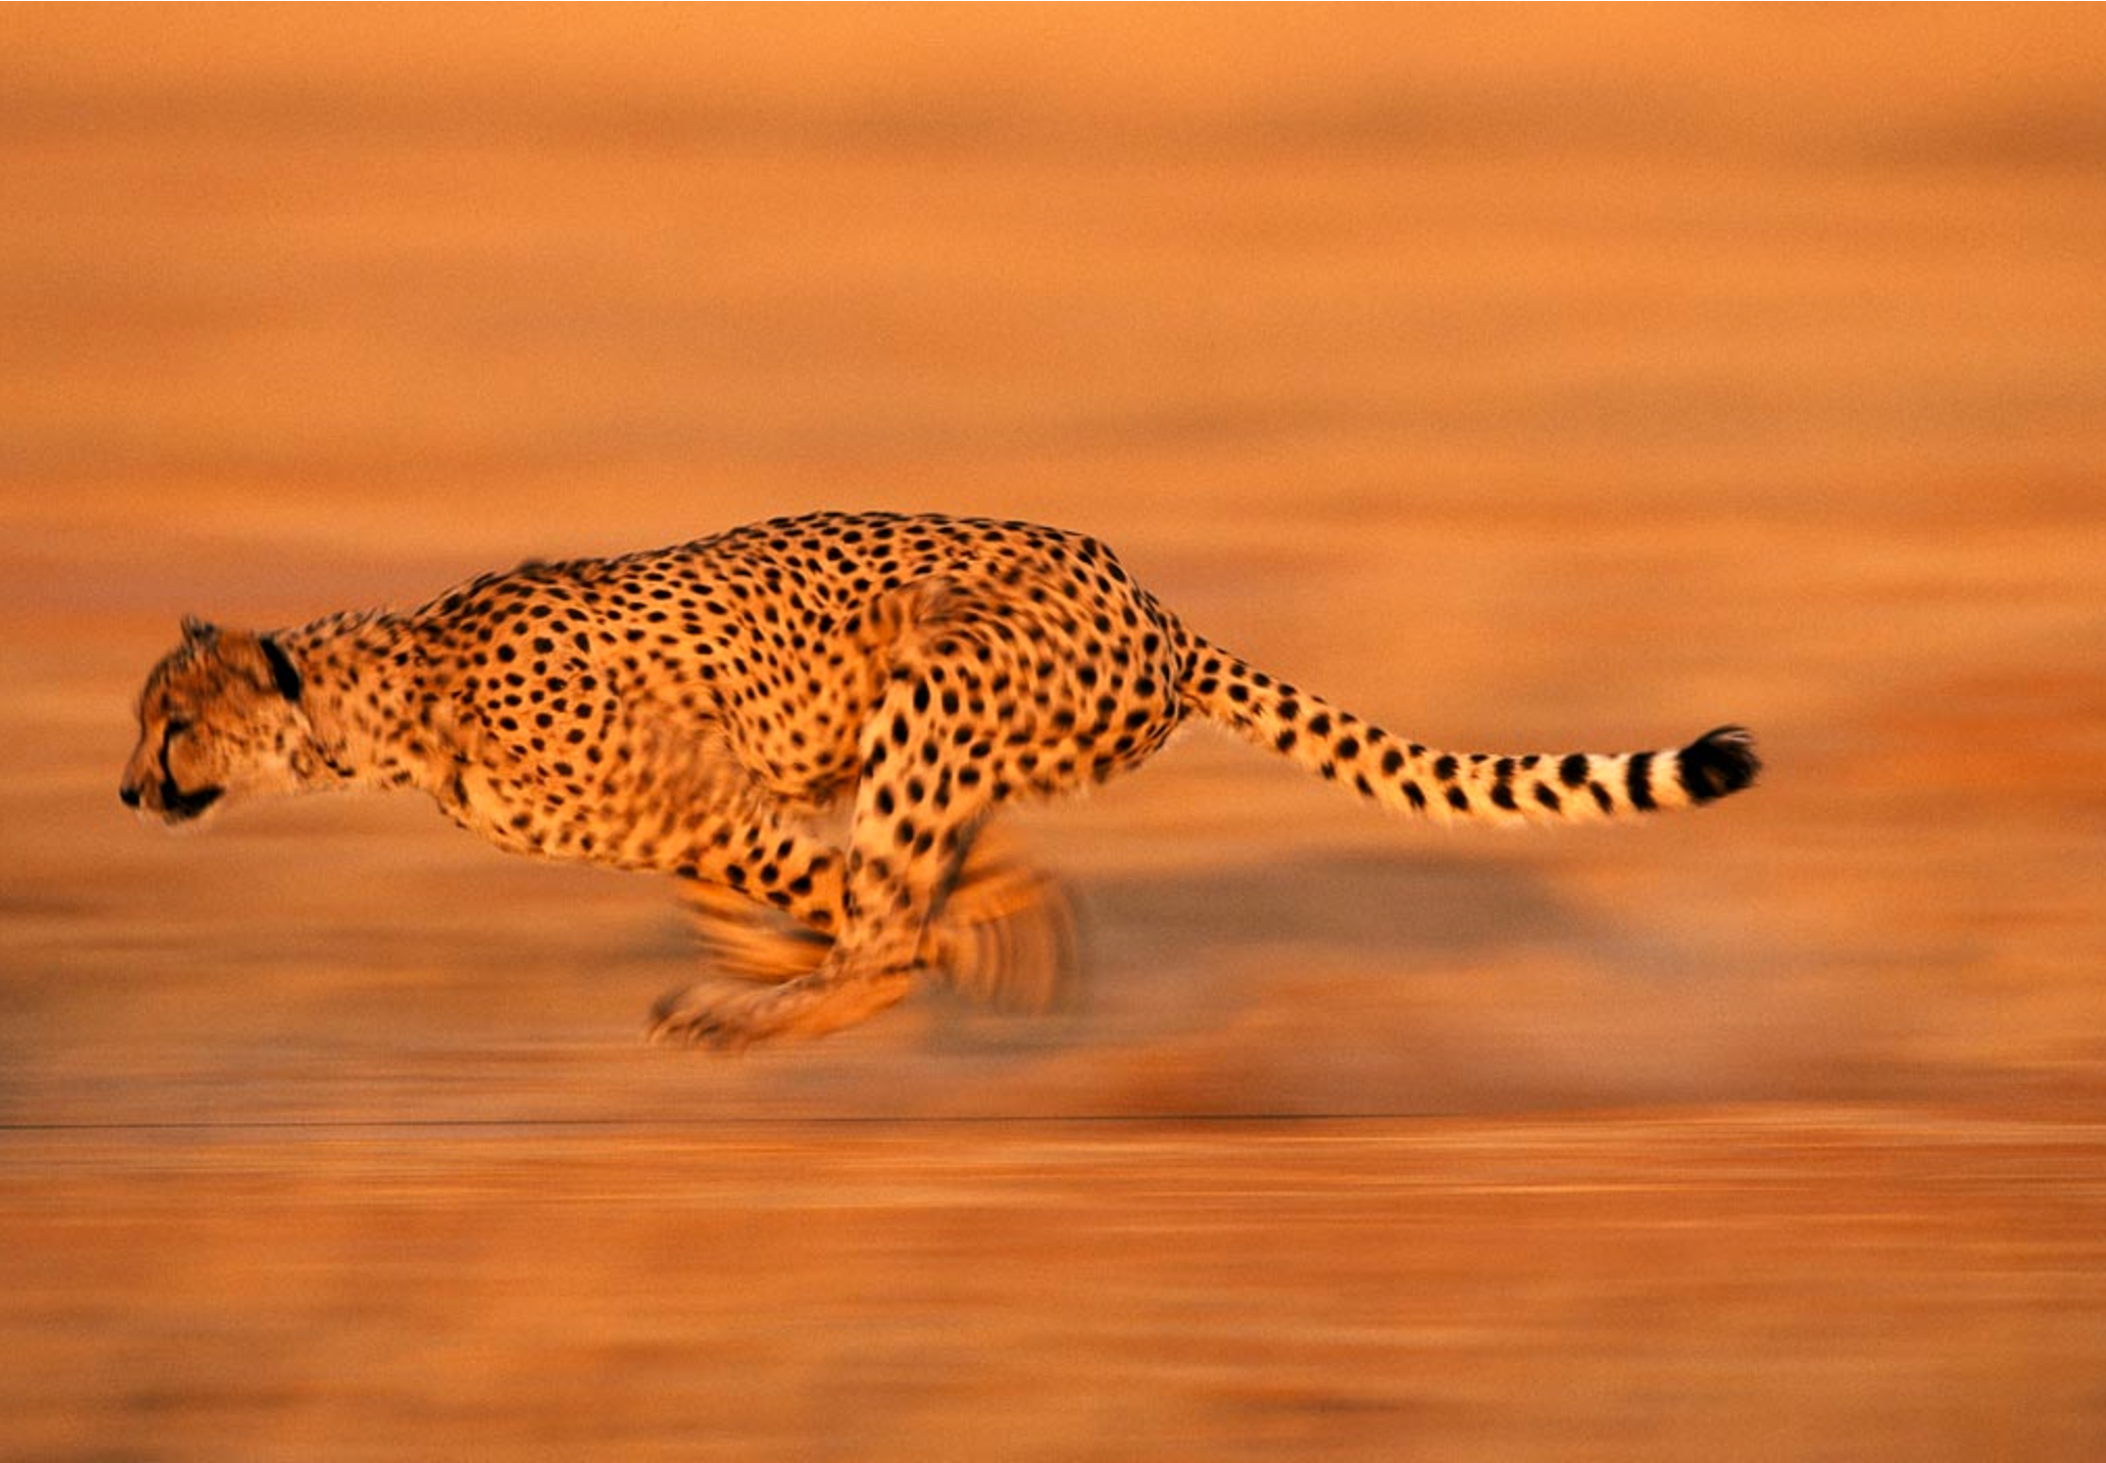
\includegraphics[trim = 0mm 0mm 0mm 0mm, clip,width=0.4\linewidth]{cheetah.pdf}}

vs.

\centering{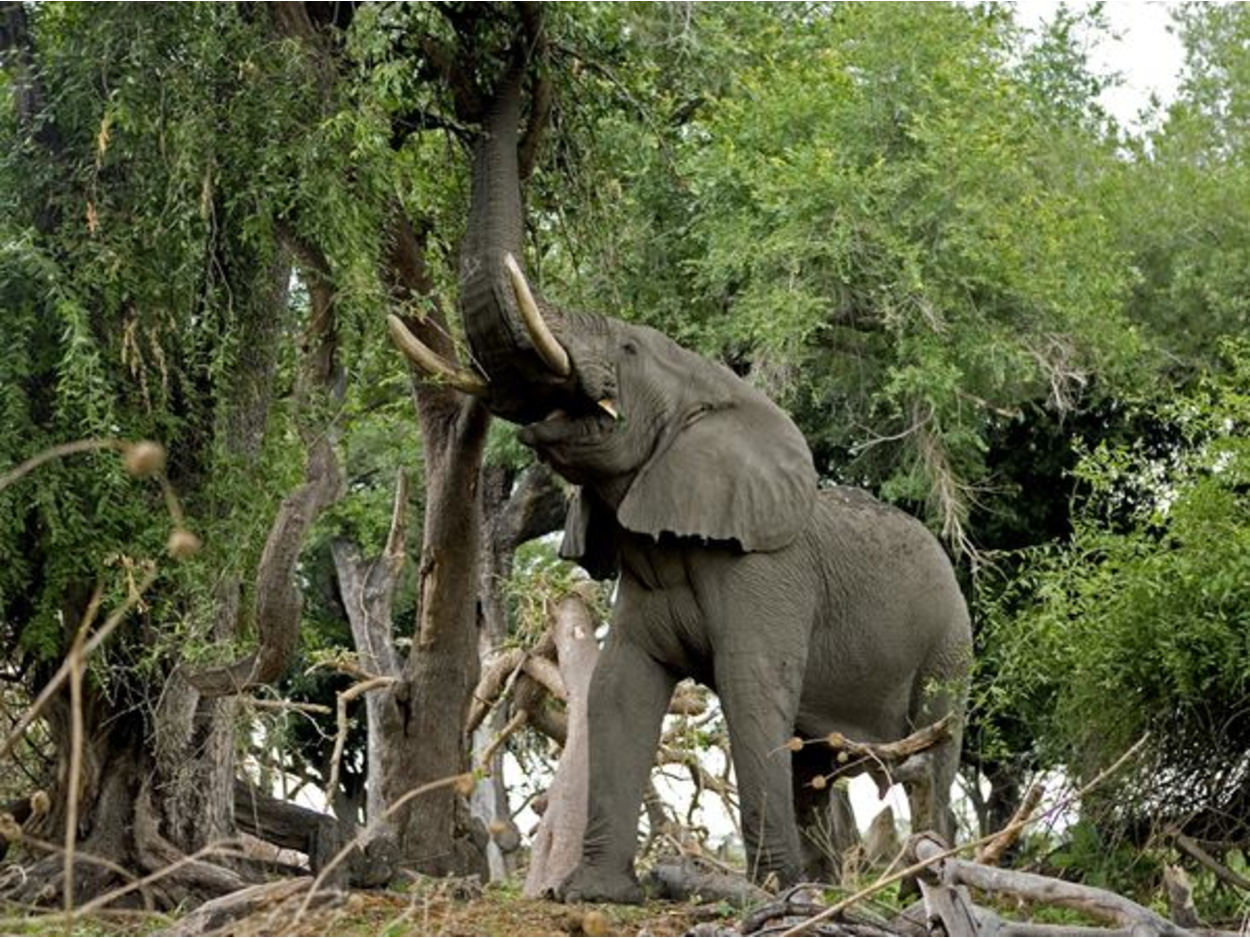
\includegraphics[trim = 0mm 0mm 0mm 0mm, clip,width=0.4\linewidth]{elephant.pdf}}

}

%\only<2>{
%\centering{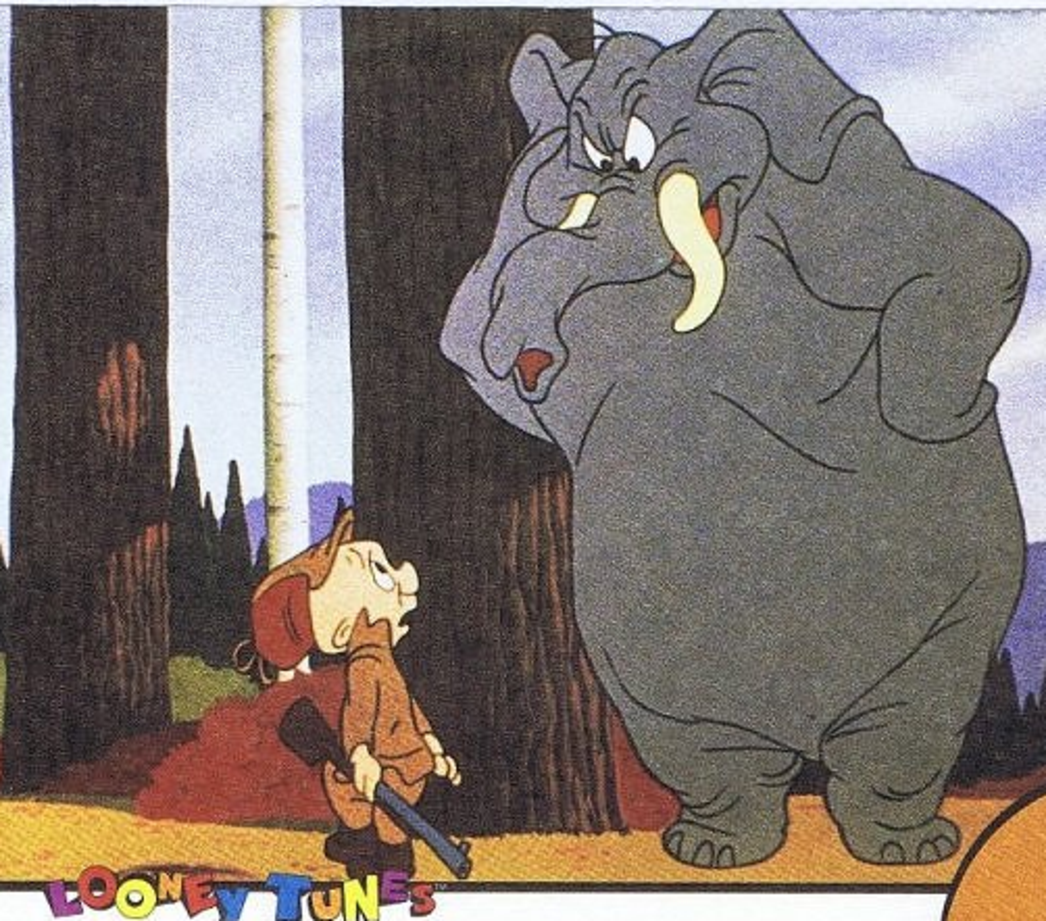
\includegraphics[trim = 0mm 0mm 0mm 0mm, clip,width=0.4\linewidth]{elephant2.pdf}}

%}

\end{frame}
%%% New Slide %%%%
\begin{frame}{Phytoplankton traits}

\only<1>{

\begin{columns}[t]

\begin{column}{0.5\linewidth}

\begin{block}

for each of these axes a whole hierarchy of traits exists that allow phytoplankton to survive and reproduce in the environment

\end{block}

\end{column}

\begin{column}{0.5\linewidth}

\centering{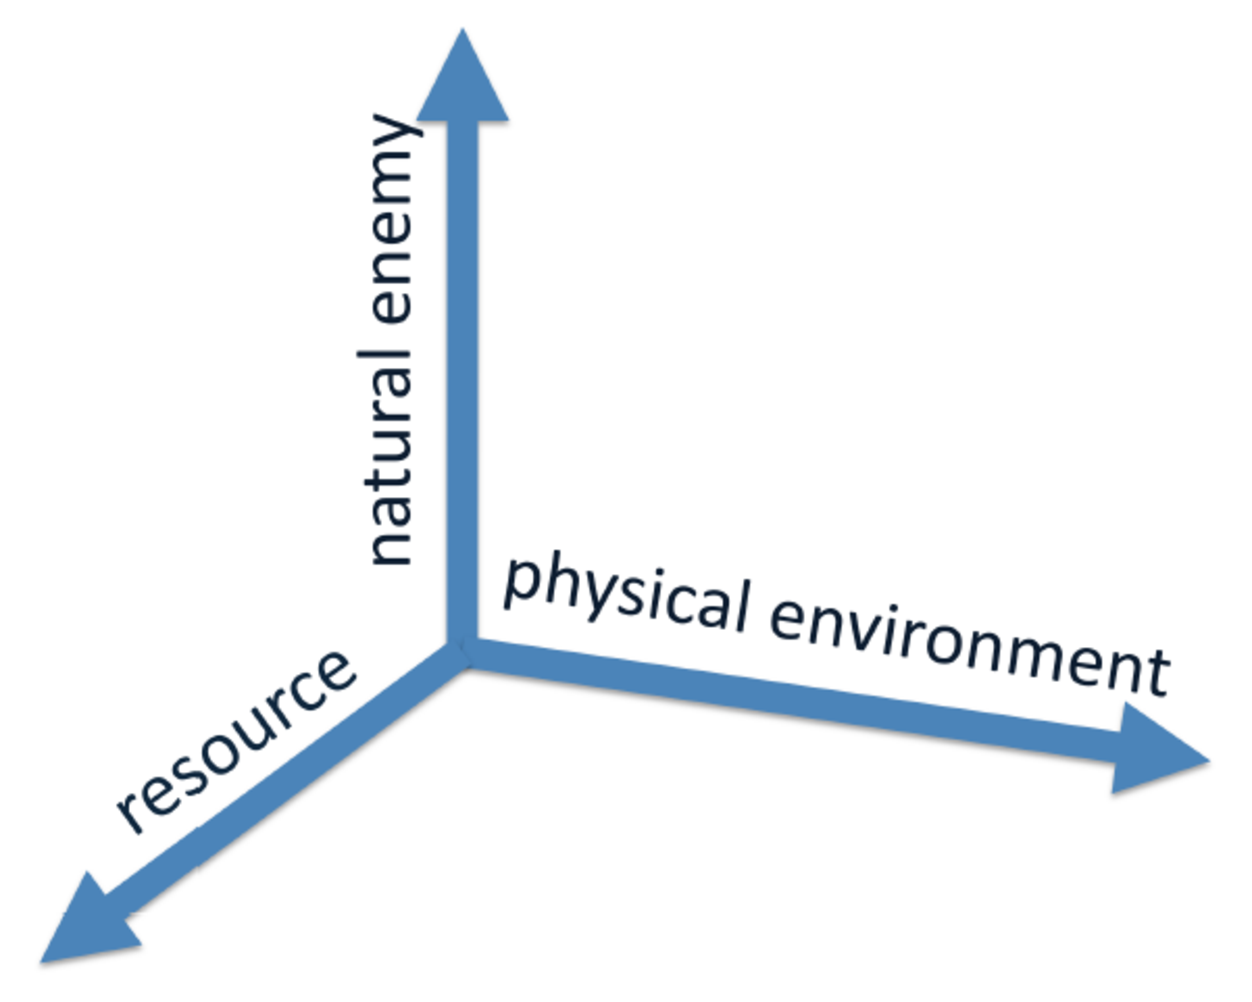
\includegraphics[width=1\textwidth]{axis.pdf}}

\end{column}

\end{columns}

}

\only<2>{

\centering{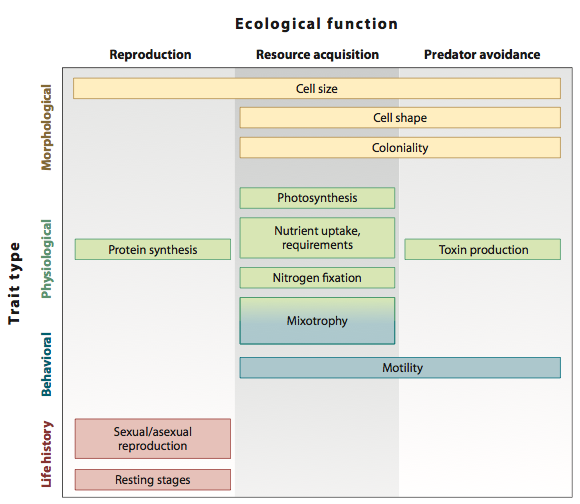
\includegraphics[width=0.65\textwidth]{Fig_litchman2008.png}}

\raggedleft {\tiny {Litchman et. al., 2008}}

}

\end{frame}
%%% New Slide %%%%
\begin{frame}{Cell size}

\centering{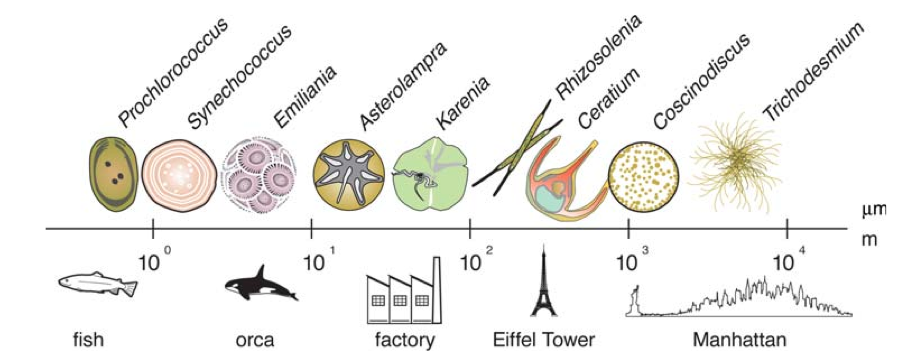
\includegraphics[width=0.9\textwidth]{Fig_finkel2009.png}}

\raggedleft {\tiny {Finkel et. al., 2009}}

\end{frame}
%%% New Slide %%%%
\begin{frame}{Cell size vs. growth}

\centering{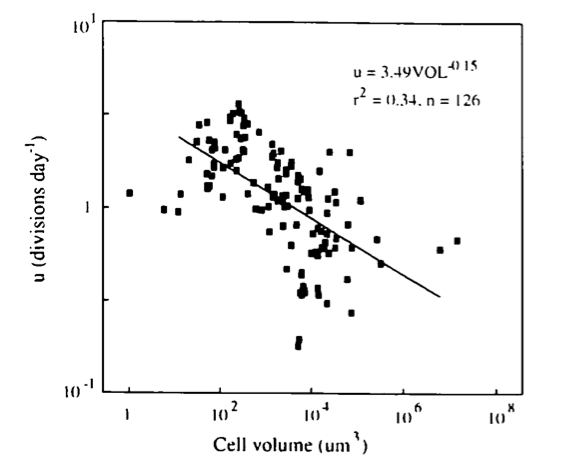
\includegraphics[width=0.6\textwidth]{Fig_tang1995.png}}

\begin{center}
\alert{smaller phytoplankton grows faster}
\end{center}

\raggedleft {\tiny {Tang, 1995}}

\end{frame}
%%% New Slide %%%%
\begin{frame}{Cell size vs. nutrients}

\centering{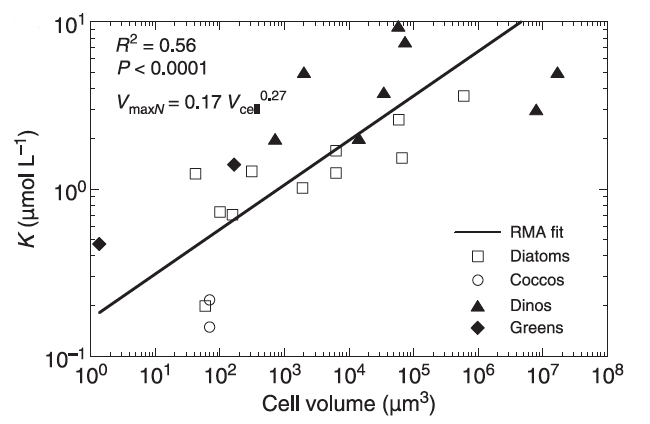
\includegraphics[width=0.6\textwidth]{litchman2007.png}}

\begin{center}
\alert{smaller phytoplankton requires less nutrients}
\end{center}

\raggedleft {\tiny {Litchman et al., 2007}}

\end{frame}
%%% New Slide %%%%
\begin{frame}{Cell size vs. photosynthesis}

\centering{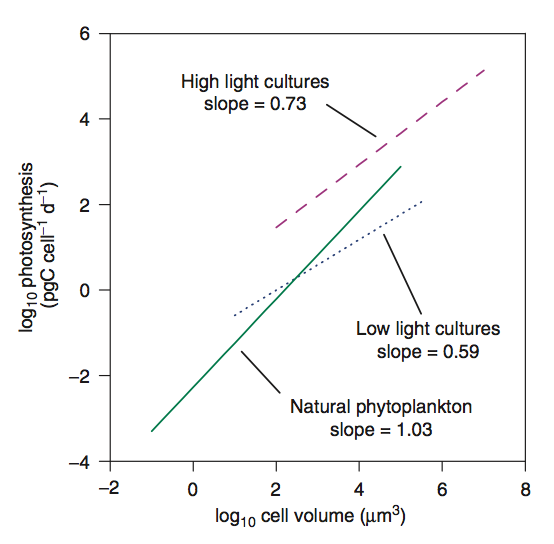
\includegraphics[width=0.5\textwidth]{Fig_maranon2009a.png}}

\begin{center}
\alert{smaller phytoplankton photosynthesizes more efficiently}
\end{center}

\raggedleft {\tiny {Marañón, 2009}}

\end{frame}
%%% New Slide %%%%
\begin{frame}{Importance of the environmental conditions}

\centering \alert {"Everything is everywhere, but the environment selects"}

\raggedleft {\tiny {Baas Becking, 1934}}

\centering{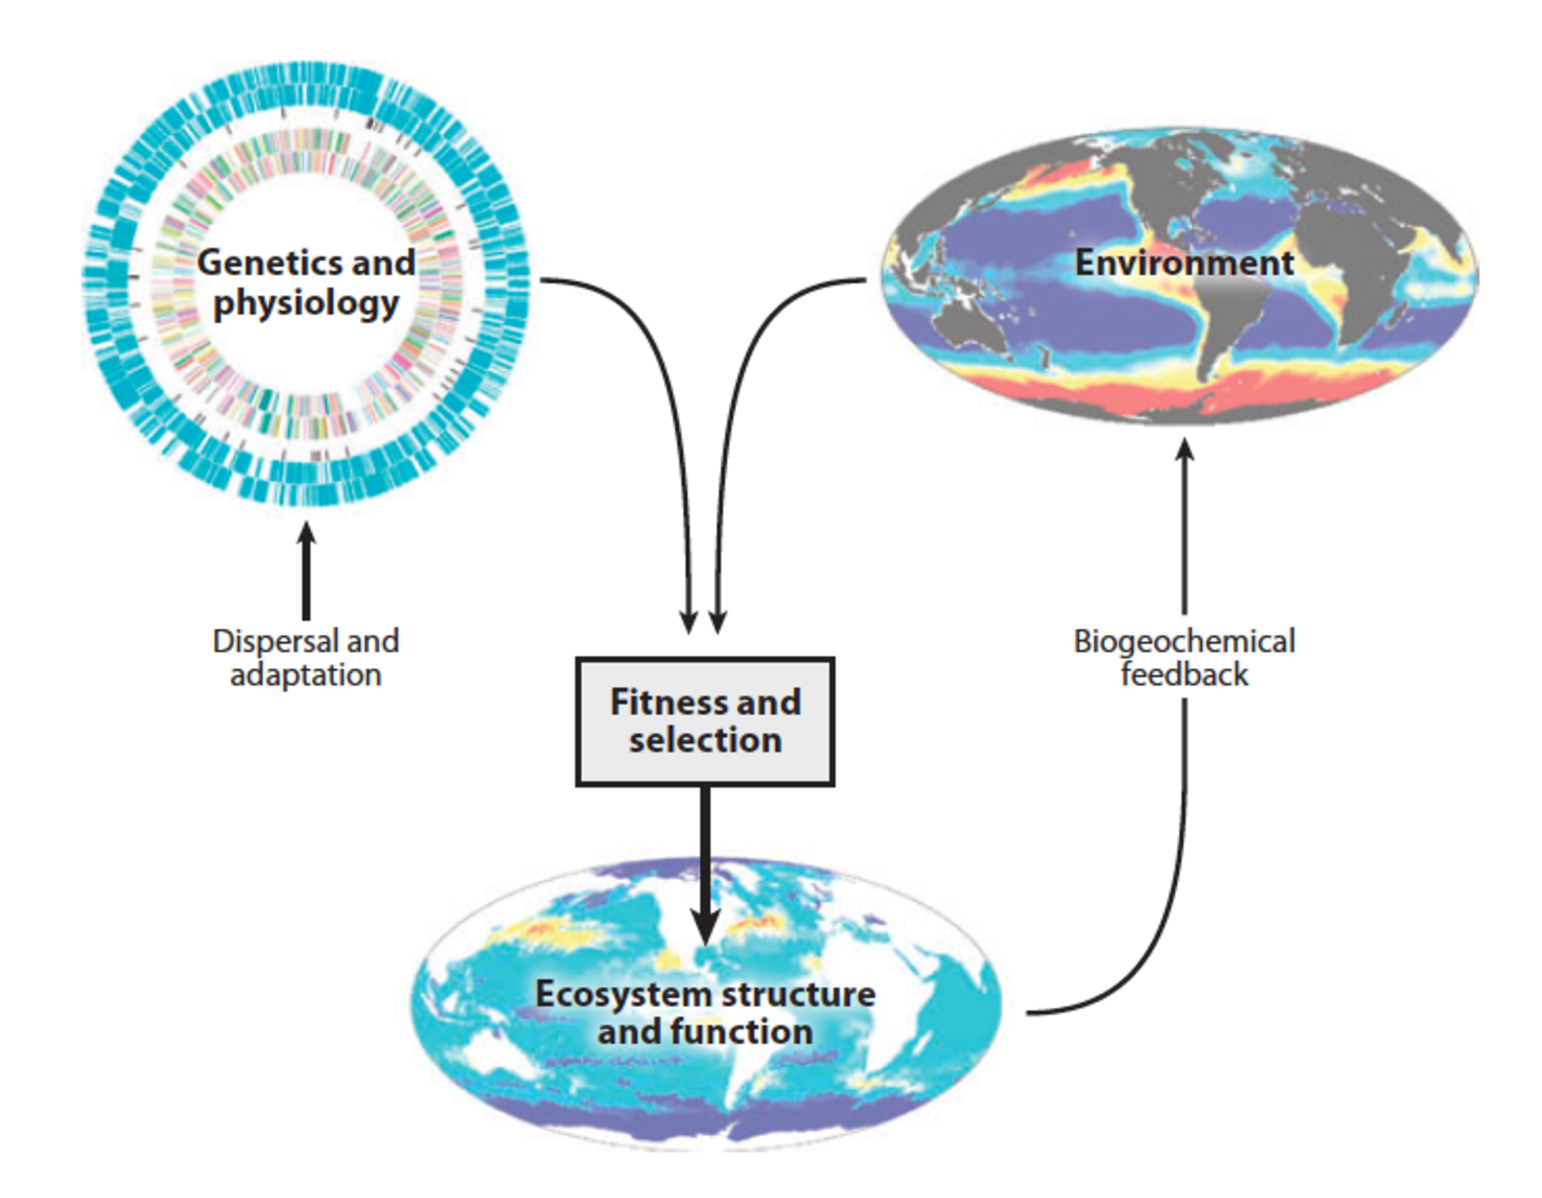
\includegraphics[width=0.6\textwidth]{follows2011.pdf}}

\raggedleft {\tiny {Follows and Dutkiewicz, 2011}}

\end{frame}
%%% New Slide %%%%
\begin{frame}{Research questions}

\begin{enumerate}
 \item {How the enviromental conditions shape the structure of phytoplankton communities?}

\vspace{0.5cm}

\pause

\item {Which are the major drivers that shape phytoplankton commuities in the Atlantic Ocean? }

\vspace{0.5cm}

\pause

\item {What is the relative contribution of bottom-up and top-down controls?}

\vspace{0.5cm}

\pause

\item {What is the relative contribution of these controls at long term environmental regimes?}

\end{enumerate}

\end{frame}
%%% New Slide %%%%
\begin{frame}{Tasks}

\begin{enumerate}
\item Select an appropriate dataset and develop a trait-based characterization of phytoplankton communities in contrasting regions of the Atlantic Ocean.
\pause 
\item Implement a size-based model to understand the factors shaping the phytoplankton community structure in contrasting regions of the Atlantic.
\pause
\item Extend the proposed size-based model to incorporate a trait-based mechanistic description also for the zooplankton community.
\pause
\item If time allows, set up the model for long-term evolutionary studies in order to understand the factors that shapes phytoplankton size evolution through geological times.
\end{enumerate}

\end{frame}

\section{Phytoplankton size-structure in the Atlantic Ocean}
%%% New Slide %%%%
\begin{frame}{Background}

\begin{columns}[t]

\begin{column}{0.7\linewidth}

The Atlantic Meridional Transect Programme

\centering{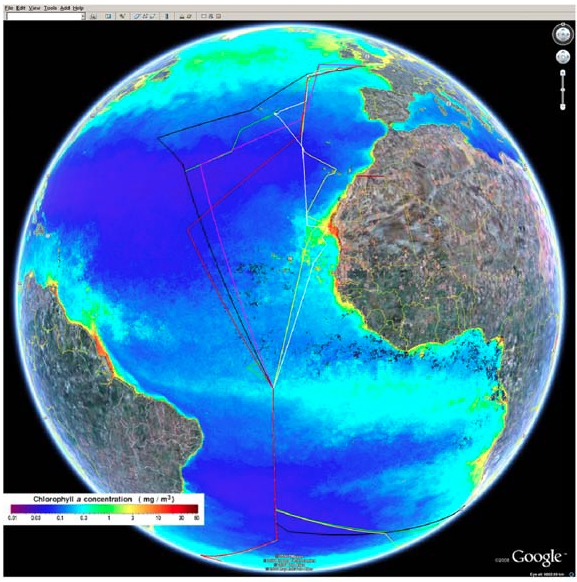
\includegraphics[width=0.7\textwidth]{robinson2009.png}}

\raggedleft {\tiny {Robinson et al., 2009}}

\end{column}

\begin{column}{0.3\linewidth}

\vspace{1cm}

\begin{itemize}

\item From 1995- until now

\item Twice a year

\item Total 21 cruises

\item Phytoplankton size-fractions, Nutrients... 

\end{itemize}

\end{column}

\end{columns}

\end{frame}
%%% New Slide %%%%
\begin{frame}{Methods}

\begin{columns}[t]

\begin{column}{0.5\linewidth}

AMT Subset

\centering{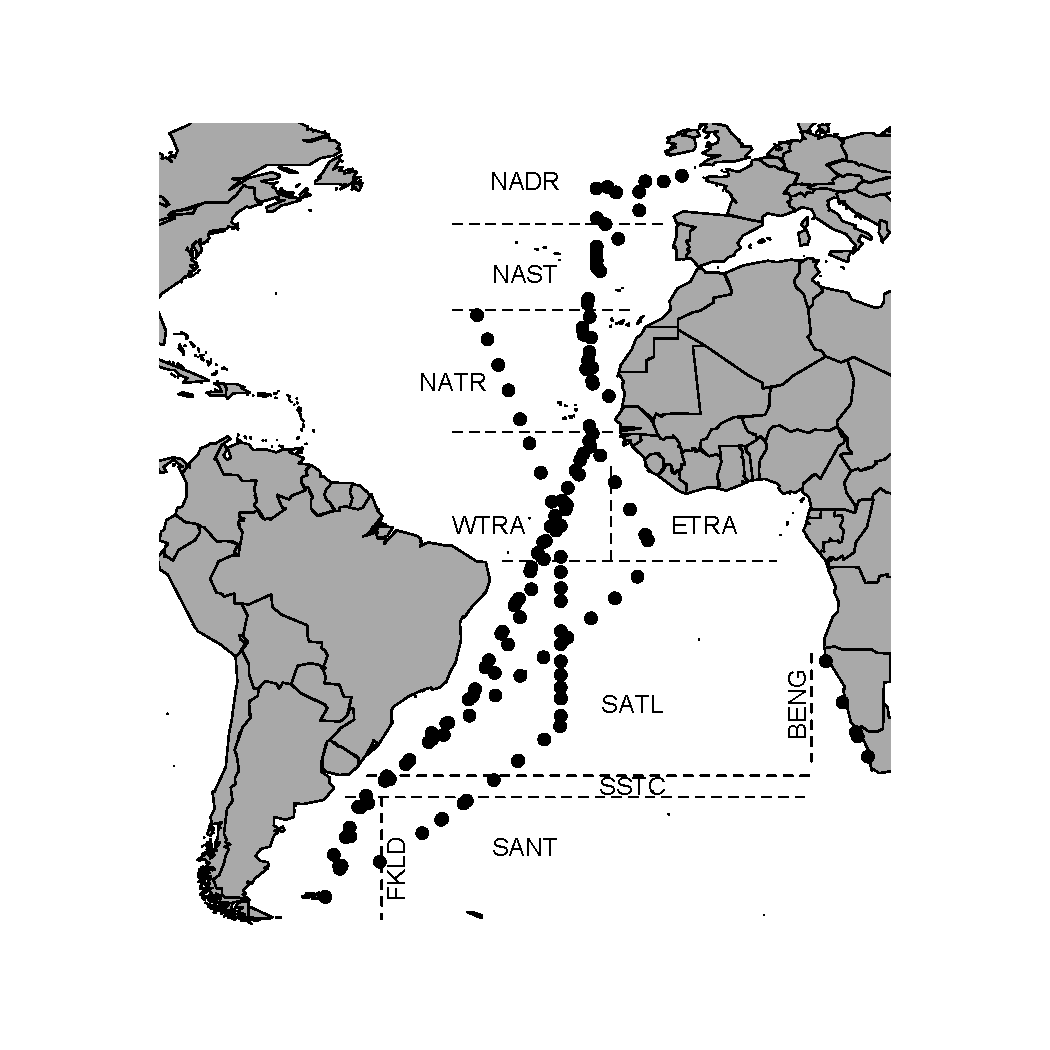
\includegraphics[trim = 20mm 10mm 20mm 20mm, clip,width=0.95\textwidth]{amt_mapFINAL2.pdf}}

\end{column}

\begin{column}{0.5\linewidth}

\begin{itemize}

\item 9 AMT cruises

\item 410 samples

\item Pico-, nano-, and microplankton

\item Longhurst (2006) classification

\item K-means classification based on nutrients and temperature

\item Environmental selection on the size-structured phytoplankton community 

\end{itemize}

\end{column}

\end{columns}

\end{frame}
%%% New Slide %%%%
\begin{frame}{Major findings}

\only<1>{

\begin{center}
Phytoplankton community structure - Longhurst
\end{center}

\centering{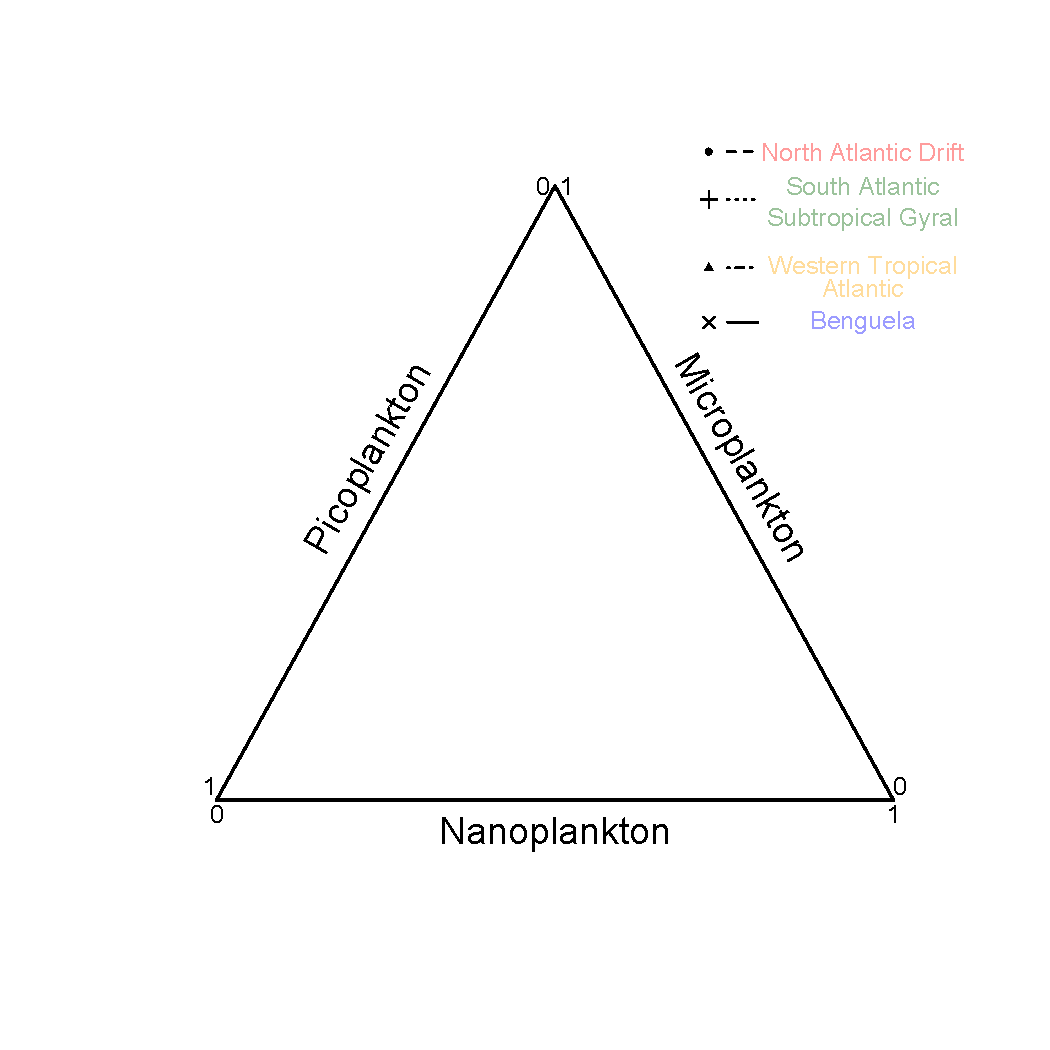
\includegraphics[trim = 10mm 10mm 10mm 10mm, clip,width=0.6\textwidth]{amt_4RegionsTriSizeFrac4-1.pdf}}

}

\only<2>{

\begin{center}
Phytoplankton community structure - Longhurst
\end{center}

\centering{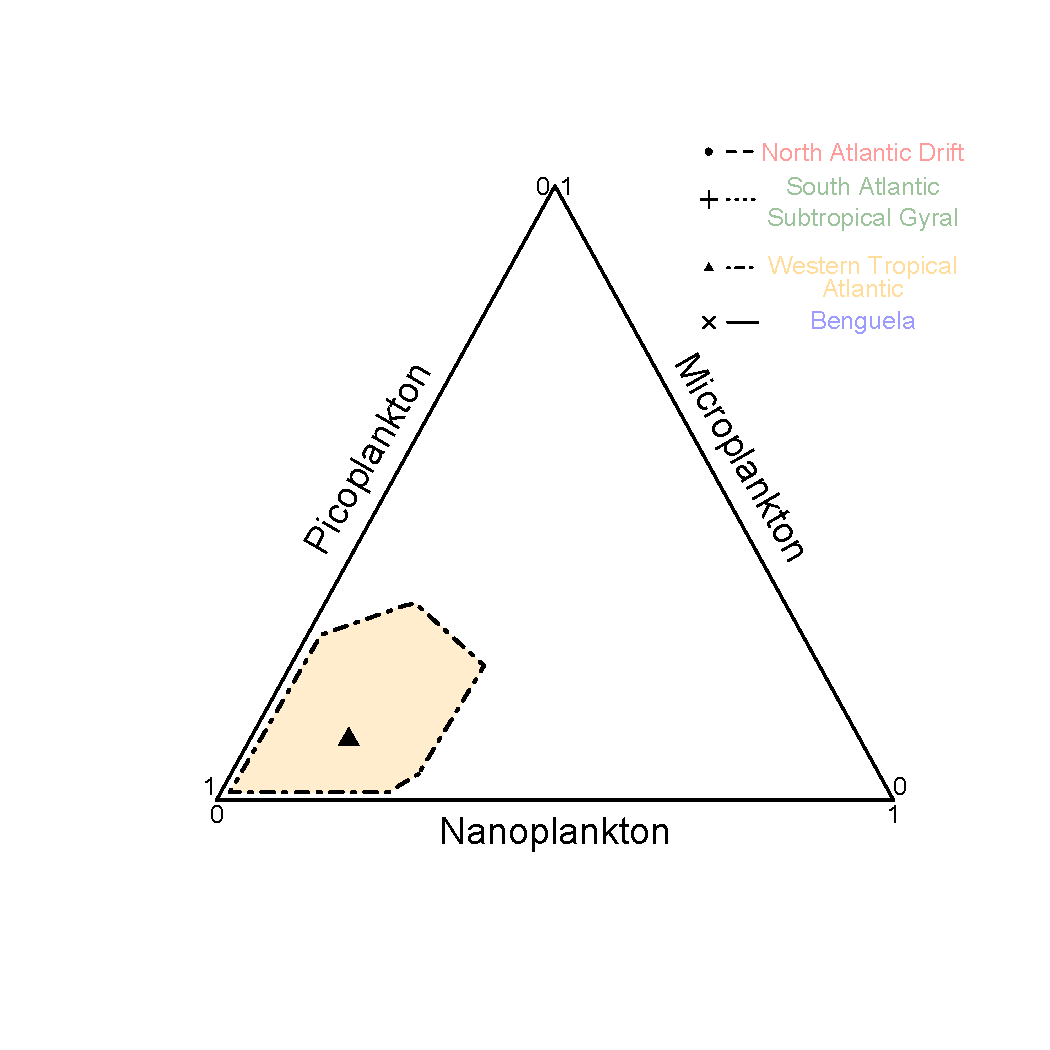
\includegraphics[trim = 10mm 10mm 10mm 10mm, clip,width=0.6\textwidth]{amt_4RegionsTriSizeFrac4-2.pdf}}

}

\only<3>{

\begin{center}
Phytoplankton community structure - Longhurst
\end{center}

\centering{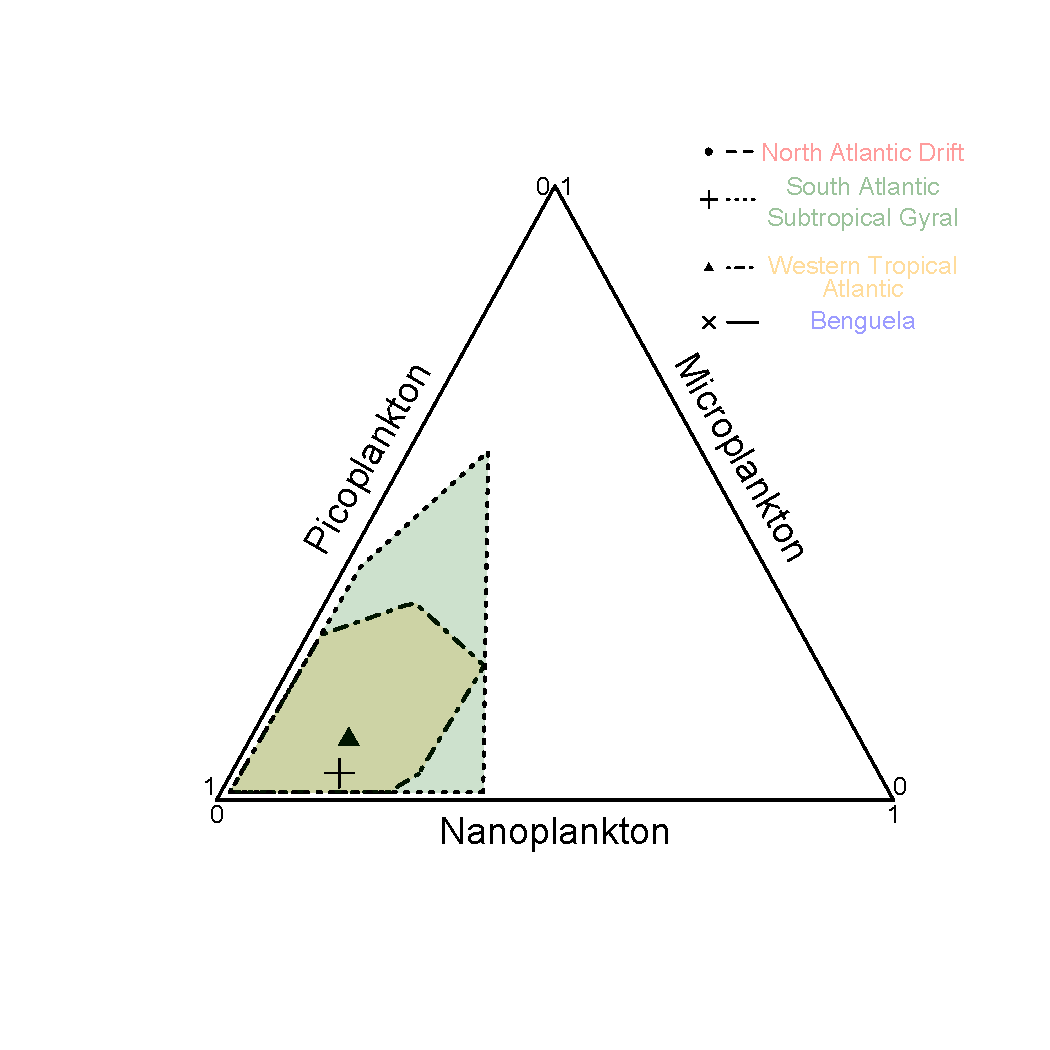
\includegraphics[trim = 10mm 10mm 10mm 10mm, clip,width=0.6\textwidth]{amt_4RegionsTriSizeFrac4-3.pdf}}

}

\only<4>{

\begin{center}
Phytoplankton community structure - Longhurst
\end{center}

\centering{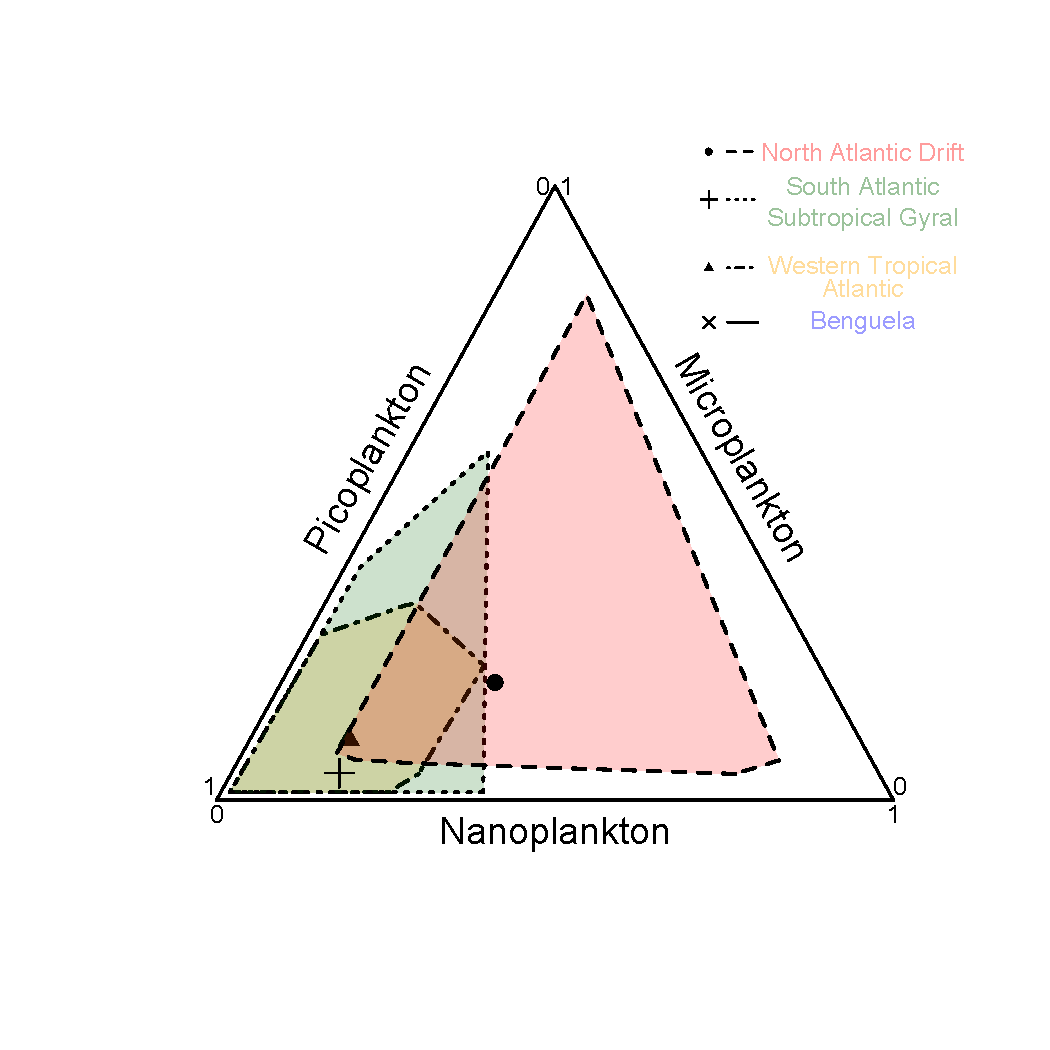
\includegraphics[trim = 10mm 10mm 10mm 10mm, clip,width=0.6\textwidth]{amt_4RegionsTriSizeFrac4-4.pdf}}

}

\only<5>{

\begin{center}
Phytoplankton community structure - Longhurst
\end{center}

\centering{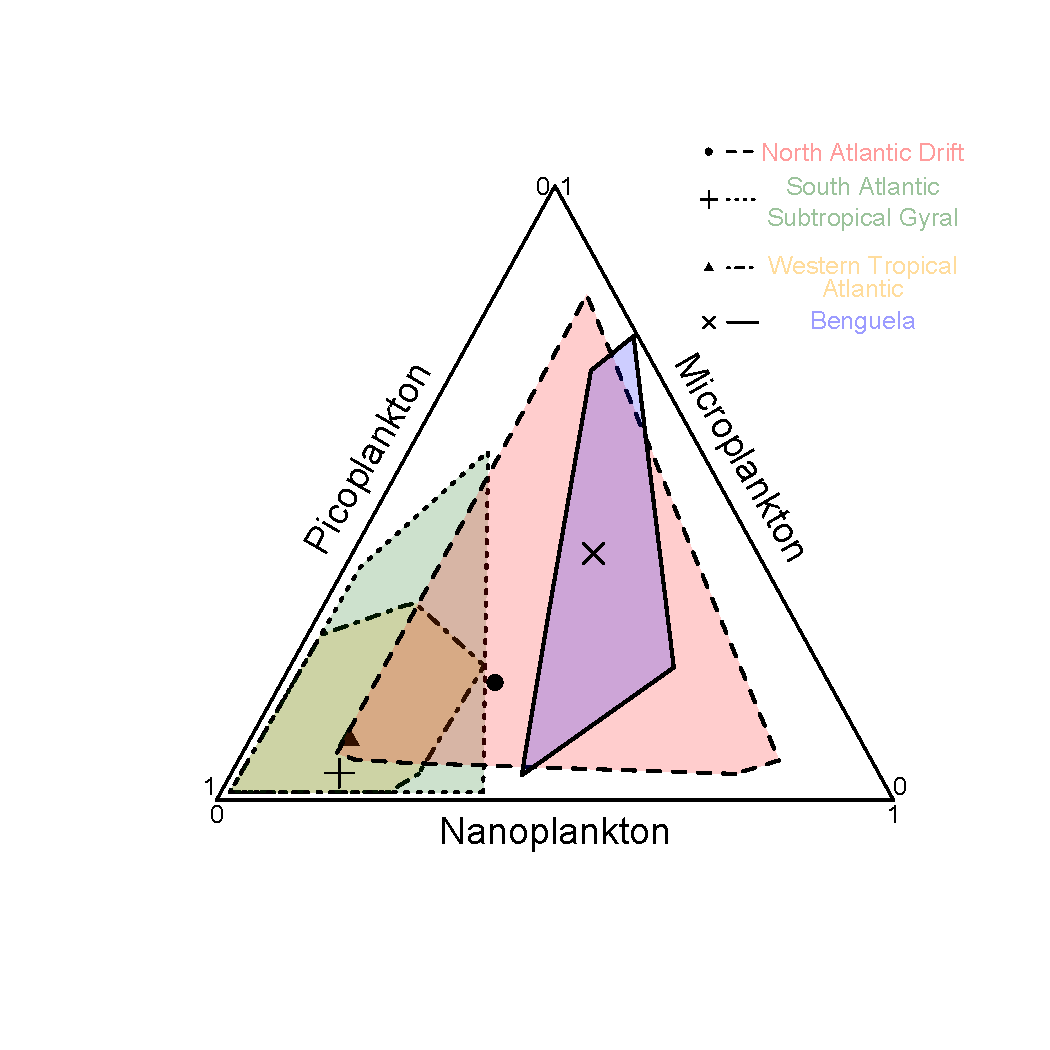
\includegraphics[trim = 10mm 10mm 10mm 10mm, clip,width=0.6\textwidth]{amt_4RegionsTriSizeFrac4-5.pdf}}

}

\only<6>{

\begin{center}
Phytoplankton community structure - Longhurst
\end{center}

\centering{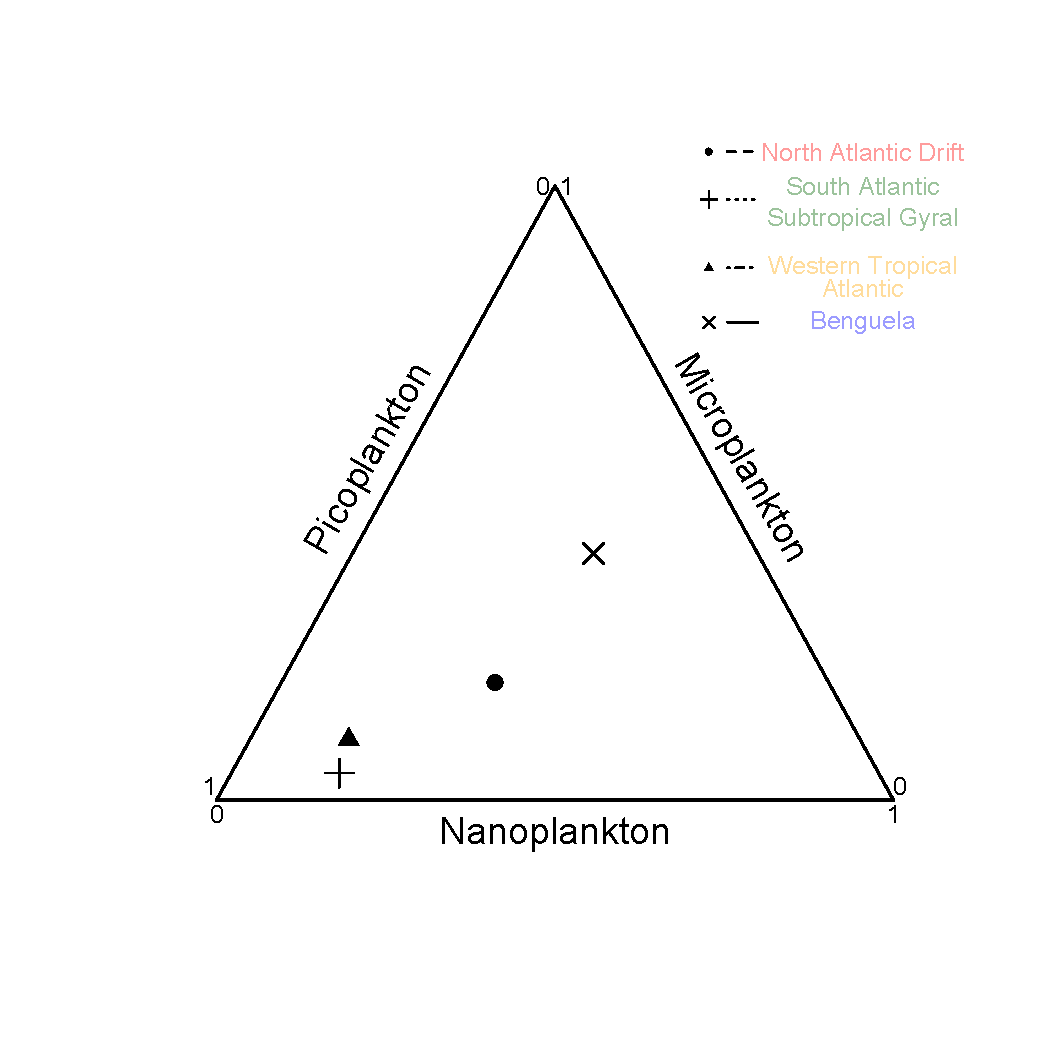
\includegraphics[trim = 10mm 10mm 10mm 10mm, clip,width=0.6\textwidth]{amt_4RegionsTriSizeFrac4-6.pdf}}

}

\end{frame}
%%% New Slide %%%%
\begin{frame}{Major findings}

\only<1>{

\begin{center}
Phytoplankton community structure - k-means clusters
\end{center}

\begin{columns}[t]

\begin{column}{0.5\linewidth}

\centering{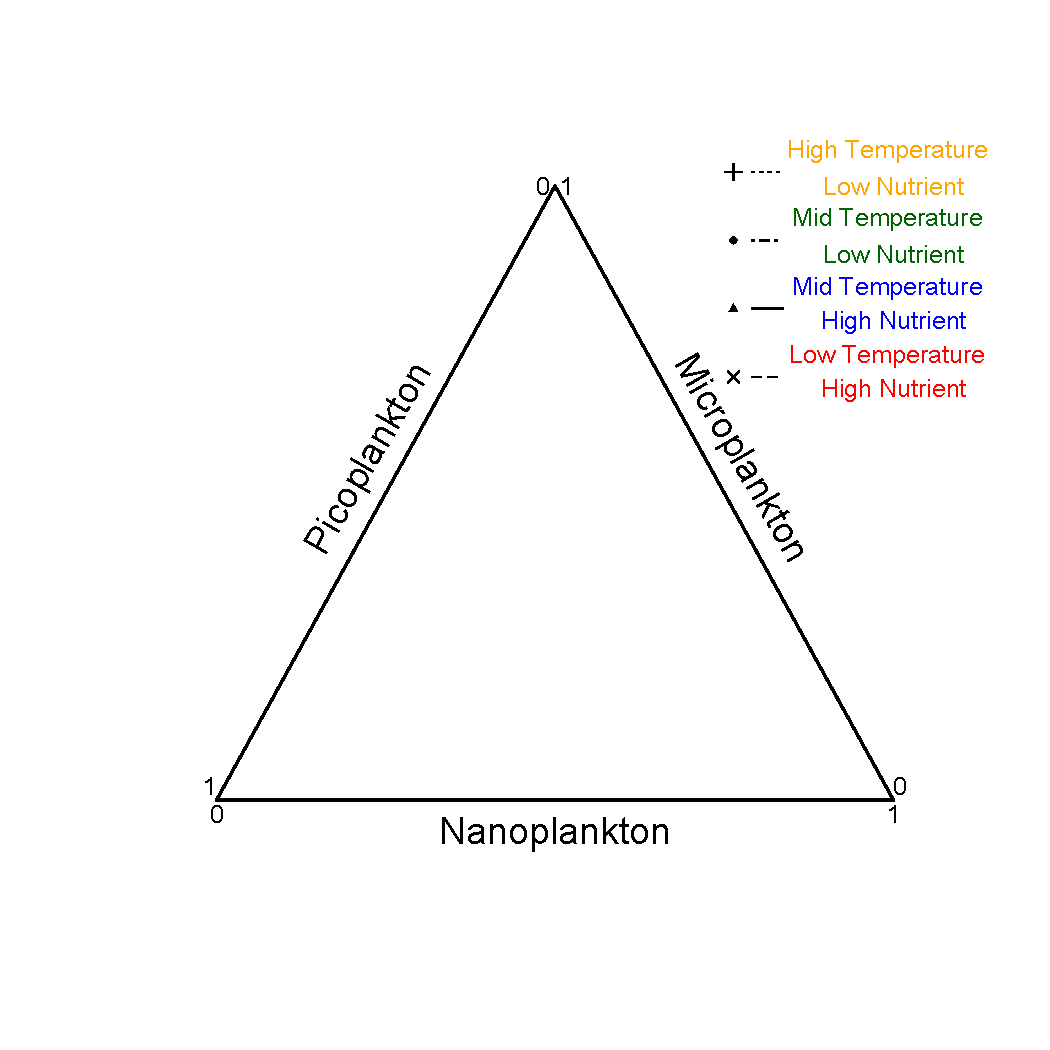
\includegraphics[trim = 10mm 10mm 10mm 10mm, clip,width=0.95\textwidth]{amt_clsEnvFINAL4-1.pdf}}

\end{column}

\begin{column}{0.5\linewidth}

\centering{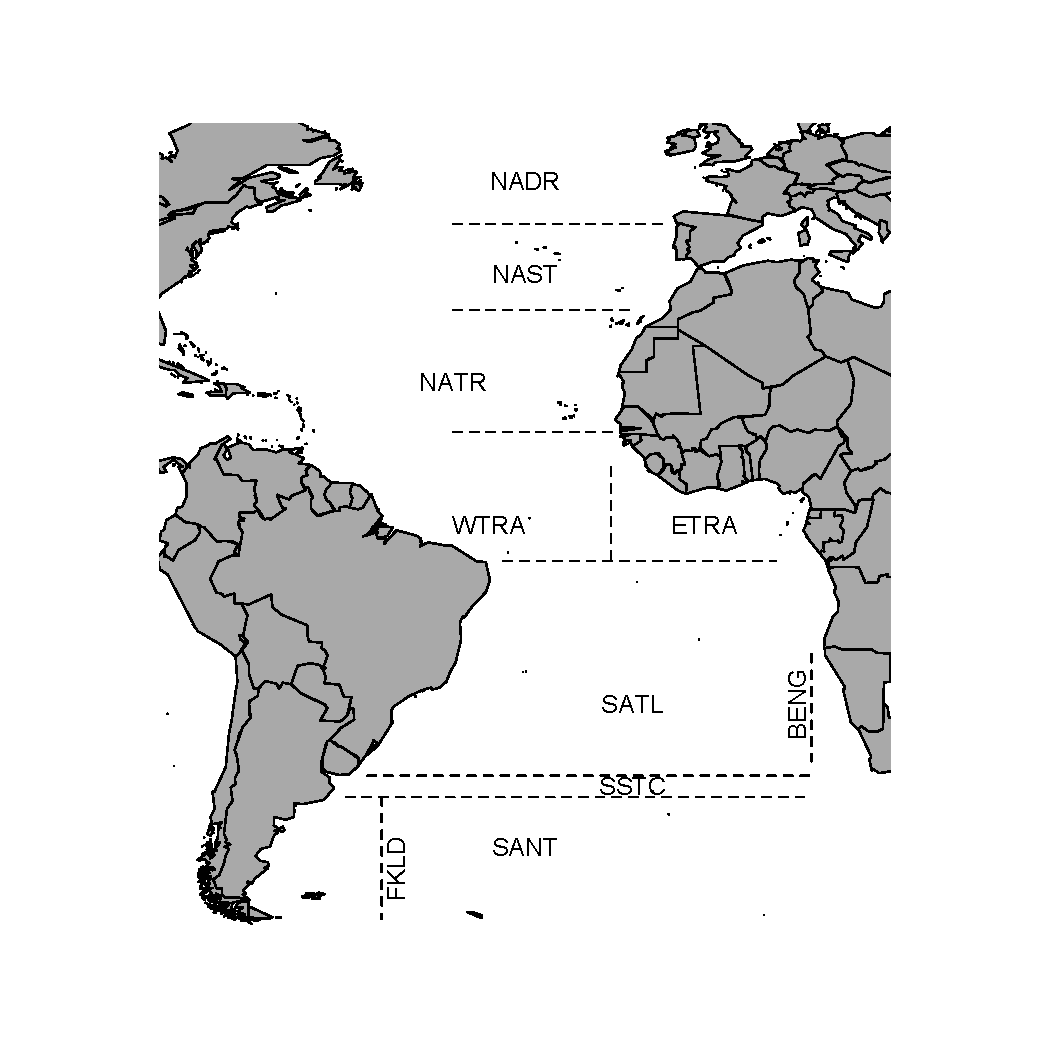
\includegraphics[trim = 20mm 10mm 20mm 20mm, clip,width=0.95\textwidth]{amt_mapClsEnv3-1.pdf}}

\end{column}

\end{columns}

}

\only<2>{

\begin{center}
Phytoplankton community structure - k-means clusters
\end{center}

\begin{columns}[t]

\begin{column}{0.5\linewidth}

\centering{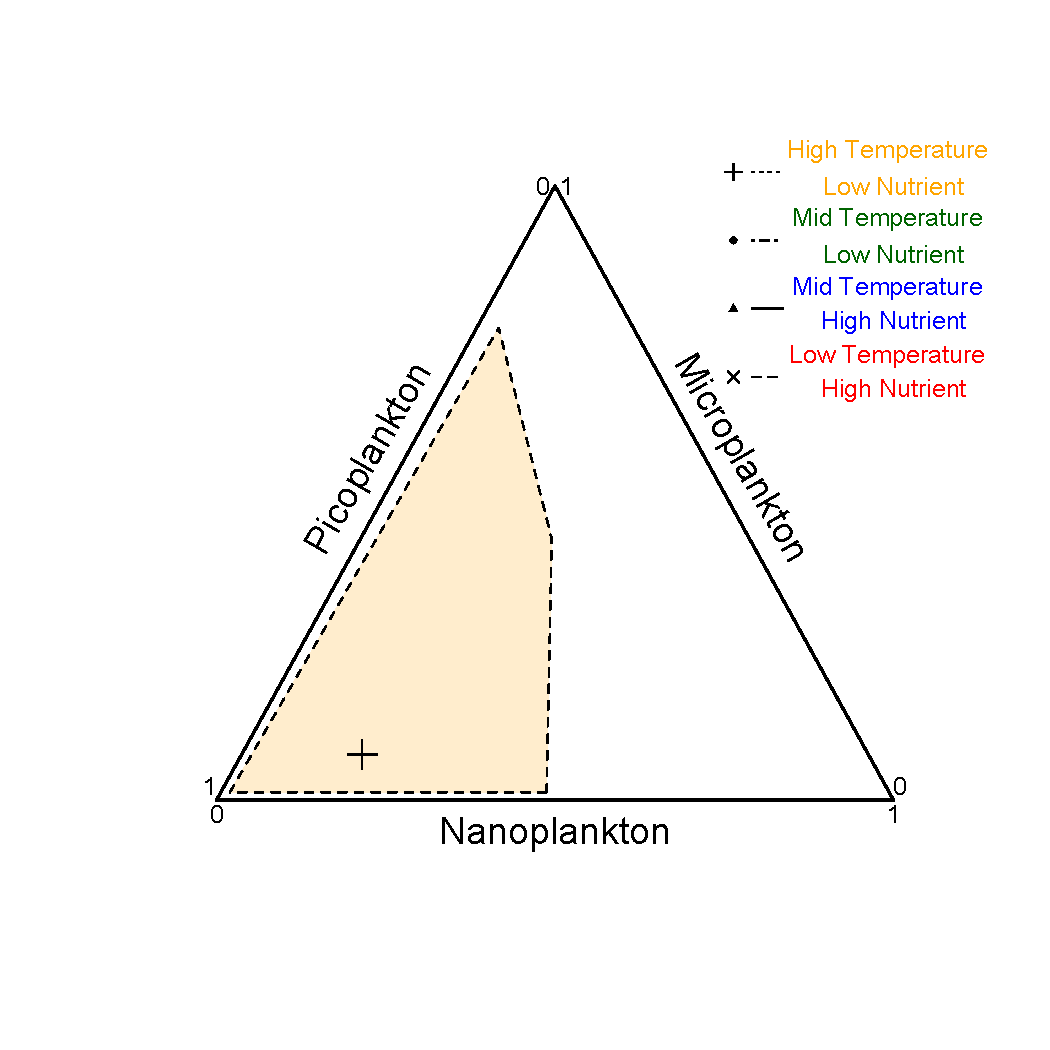
\includegraphics[trim = 10mm 10mm 10mm 10mm, clip,width=0.95\textwidth]{amt_clsEnvFINAL4-2.pdf}}

\end{column}

\begin{column}{0.5\linewidth}

\centering{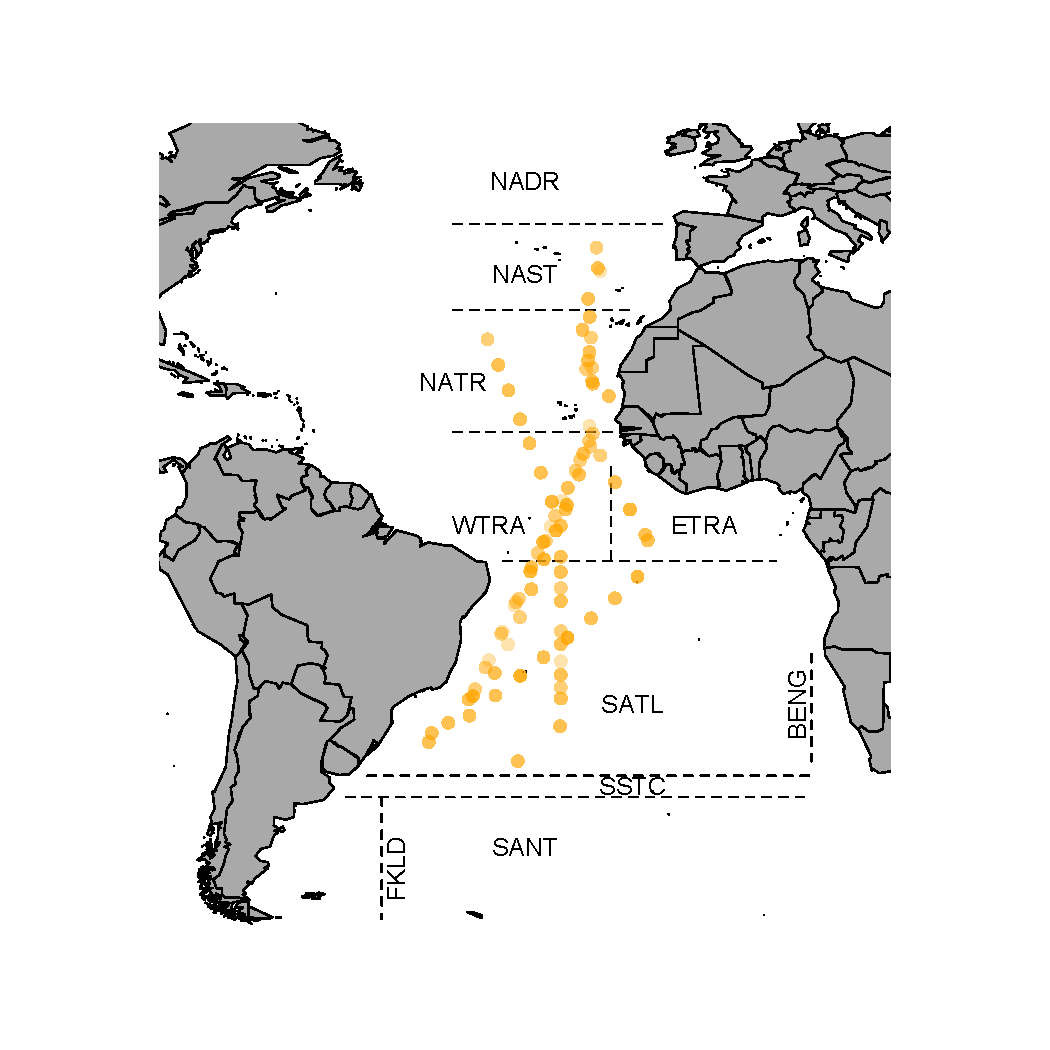
\includegraphics[trim = 20mm 10mm 20mm 20mm, clip,width=0.95\textwidth]{amt_mapClsEnv3-2.pdf}}

\end{column}

\end{columns}

}

\only<3>{

\begin{center}
Phytoplankton community structure - k-means clusters
\end{center}

\begin{columns}[t]

\begin{column}{0.5\linewidth}

\centering{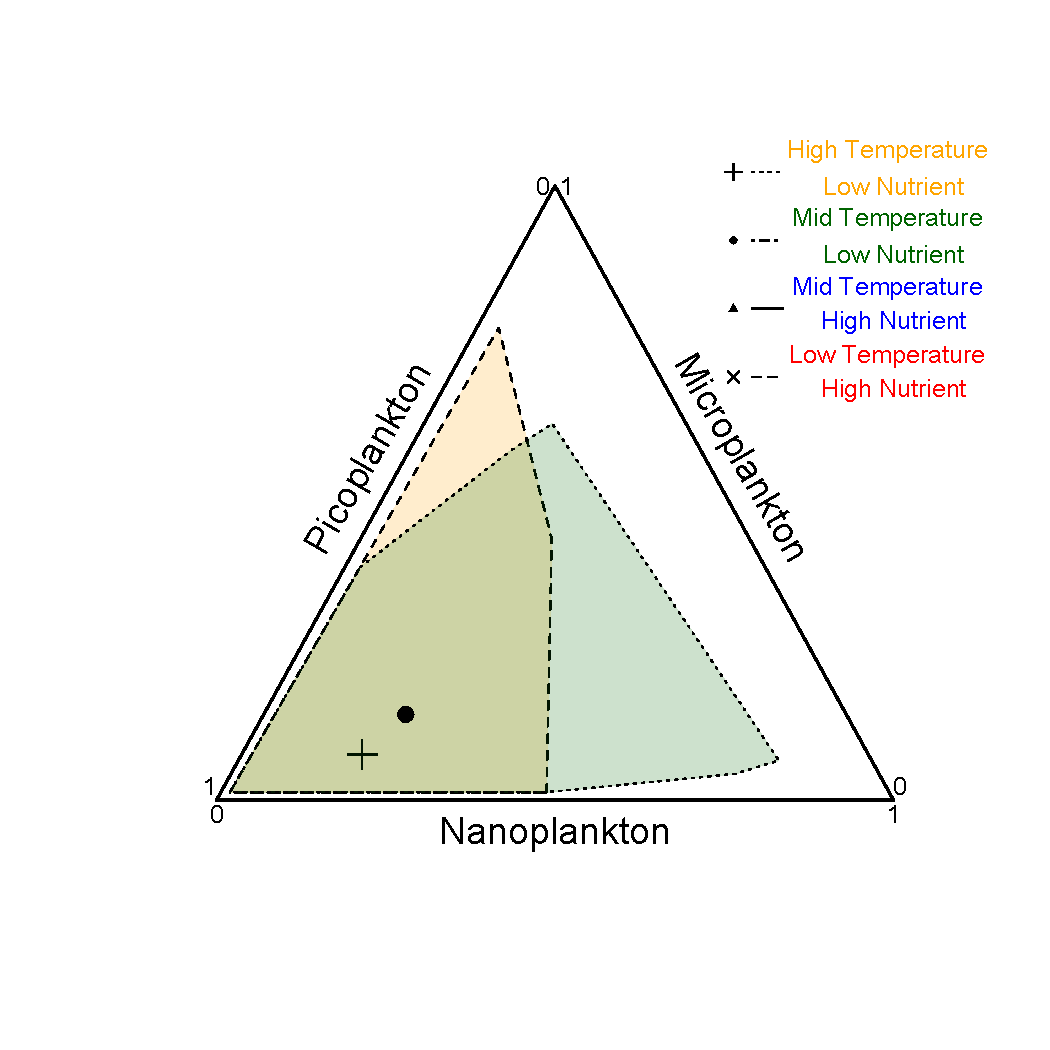
\includegraphics[trim = 10mm 10mm 10mm 10mm, clip,width=0.95\textwidth]{amt_clsEnvFINAL4-3.pdf}}

\end{column}

\begin{column}{0.5\linewidth}

\centering{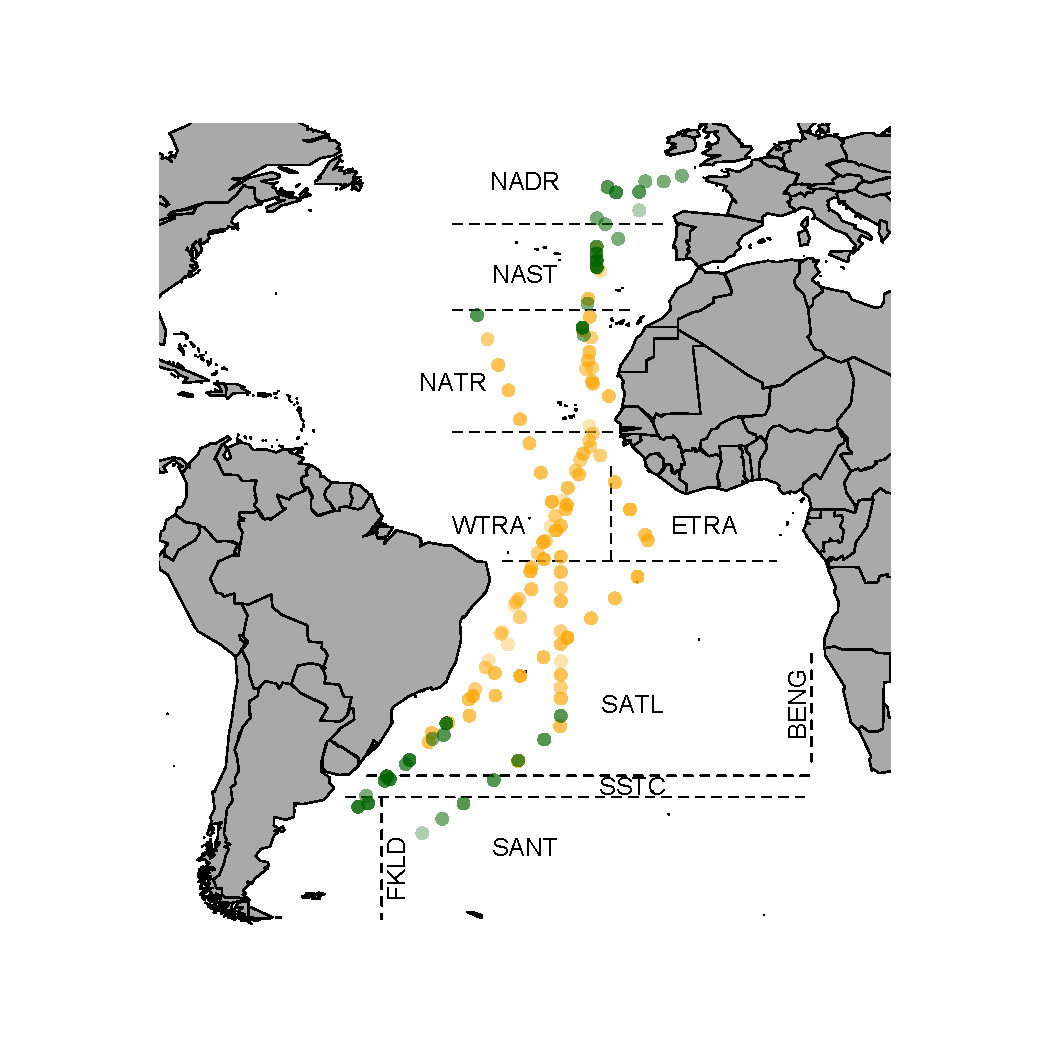
\includegraphics[trim = 20mm 10mm 20mm 20mm, clip,width=0.95\textwidth]{amt_mapClsEnv3-3.pdf}}

\end{column}

\end{columns}

}

\only<4>{

\begin{center}
Phytoplankton community structure - k-means clusters
\end{center}

\begin{columns}[t]

\begin{column}{0.5\linewidth}

\centering{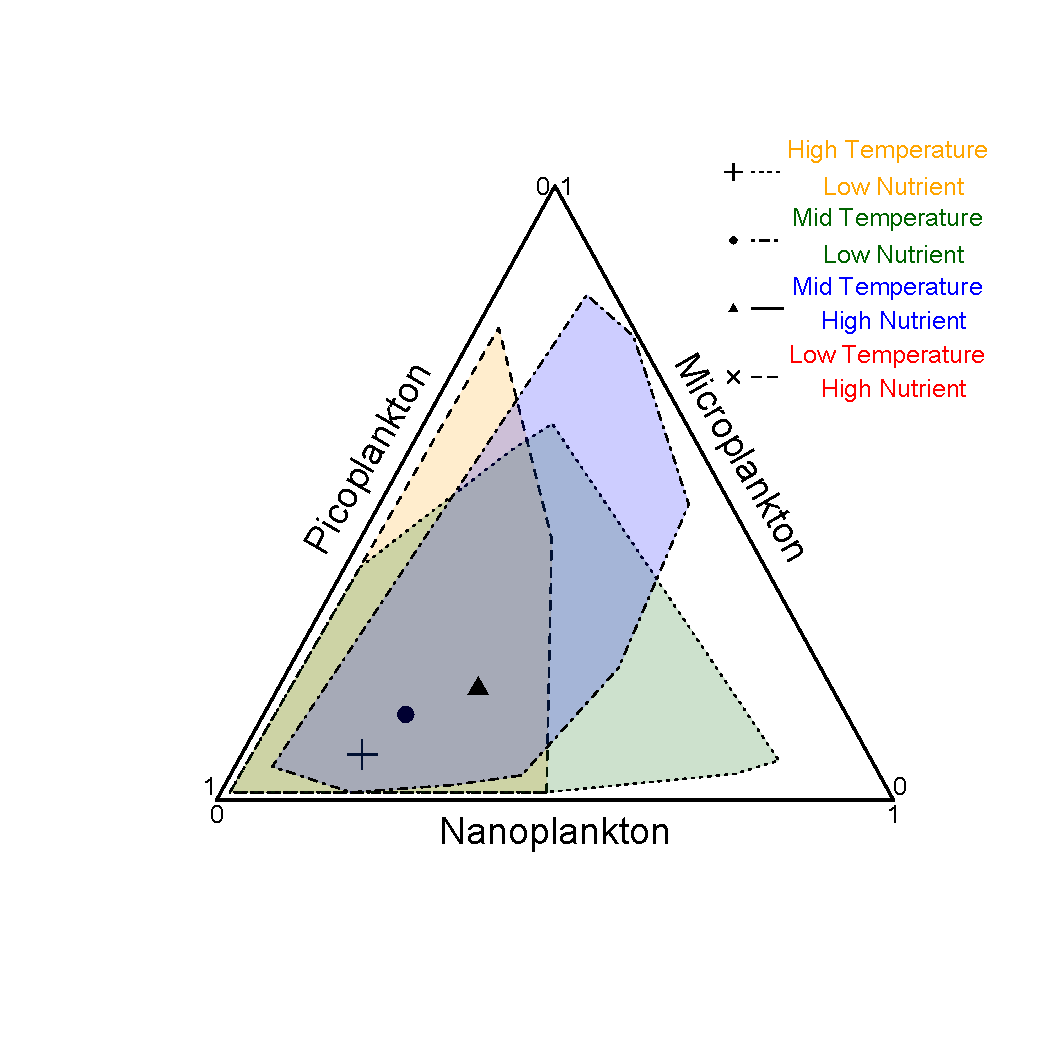
\includegraphics[trim = 10mm 10mm 10mm 10mm, clip,width=0.95\textwidth]{amt_clsEnvFINAL4-4.pdf}}

\end{column}

\begin{column}{0.5\linewidth}

\centering{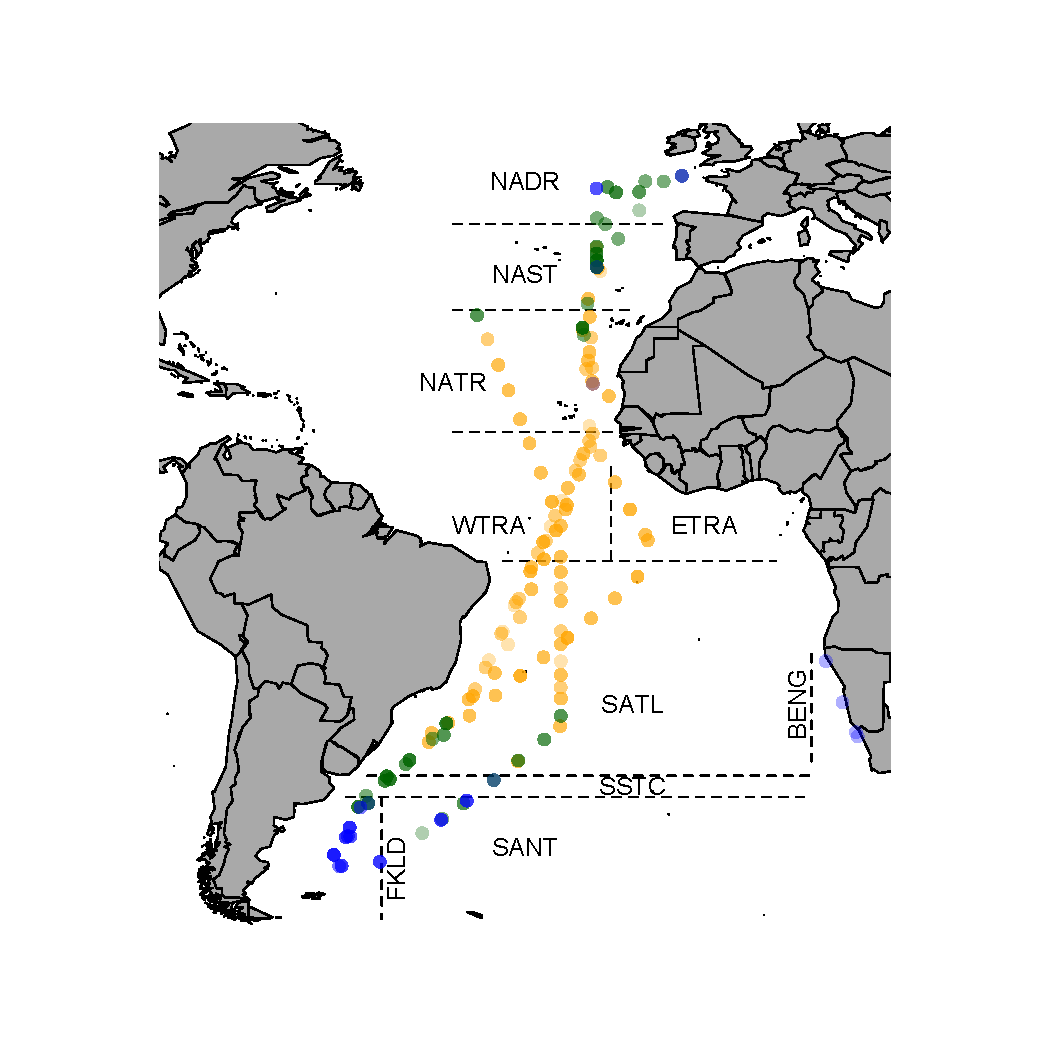
\includegraphics[trim = 20mm 10mm 20mm 20mm, clip,width=0.95\textwidth]{amt_mapClsEnv3-4.pdf}}

\end{column}

\end{columns}

}

\only<5>{

\begin{center}
Phytoplankton community structure - k-means clusters
\end{center}

\begin{columns}[t]

\begin{column}{0.5\linewidth}

\centering{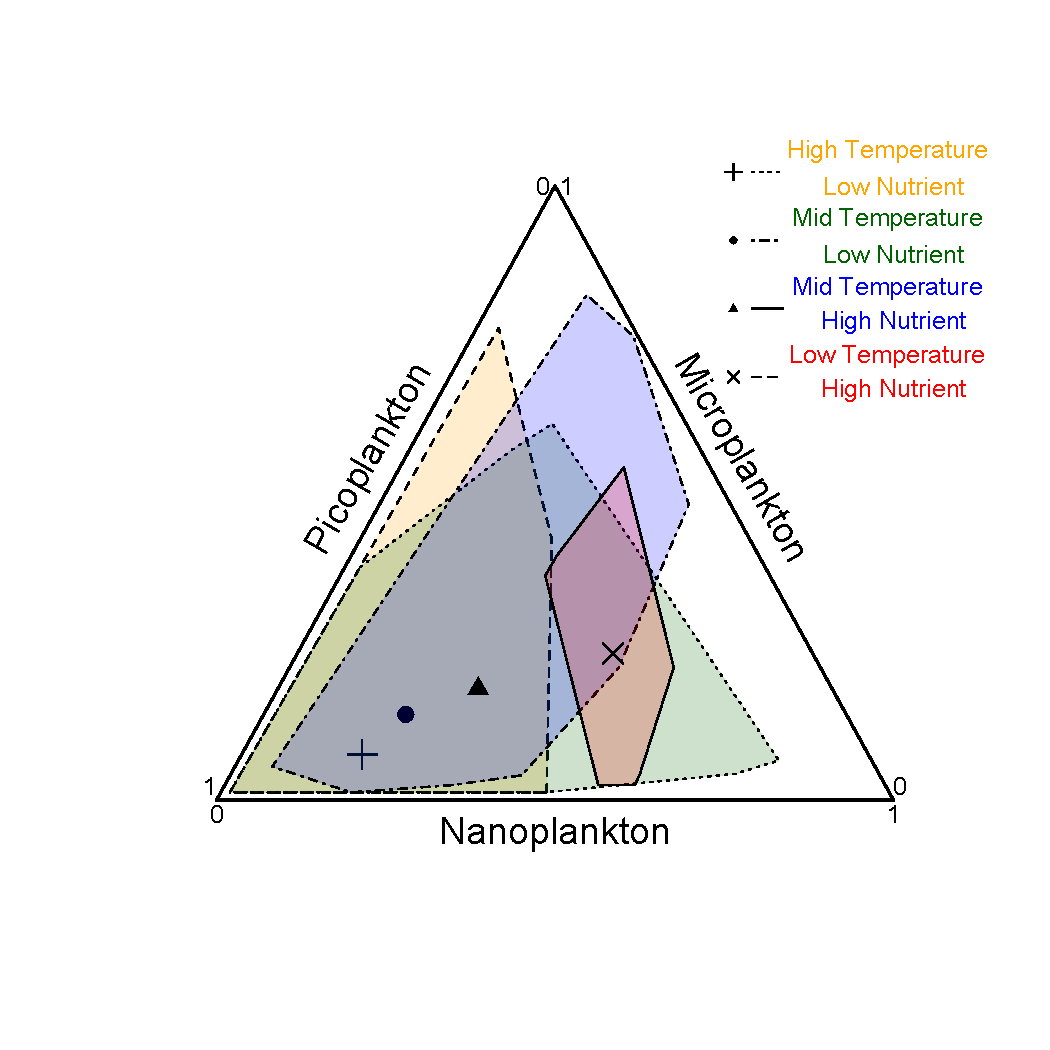
\includegraphics[trim = 10mm 10mm 10mm 10mm, clip,width=0.95\textwidth]{amt_clsEnvFINAL4-5.pdf}}

\end{column}

\begin{column}{0.5\linewidth}

\centering{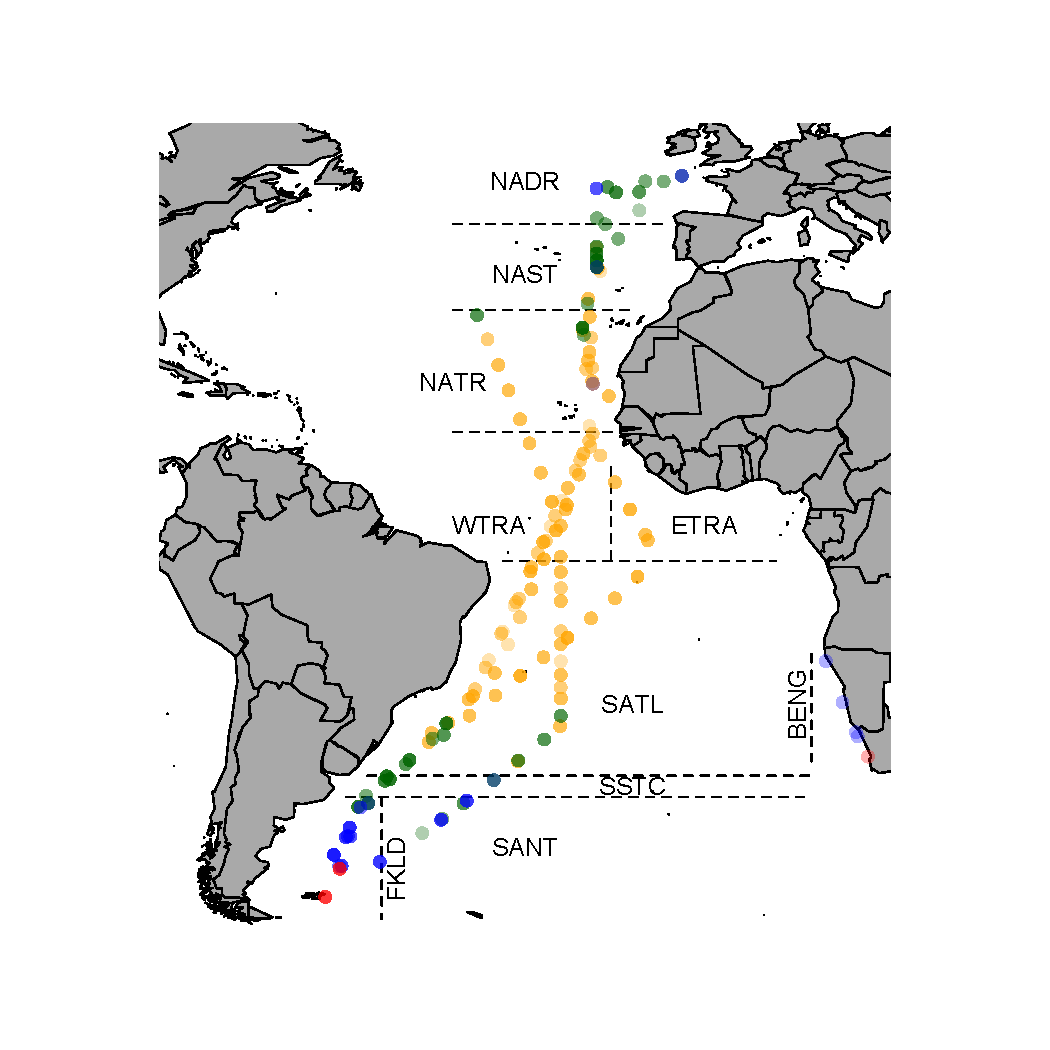
\includegraphics[trim = 20mm 10mm 20mm 20mm, clip,width=0.95\textwidth]{amt_mapClsEnv3-5.pdf}}

\end{column}

\end{columns}

}

\only<6>{

\begin{center}
Phytoplankton community structure - k-means clusters
\end{center}

\begin{columns}[t]

\begin{column}{0.5\linewidth}

\centering{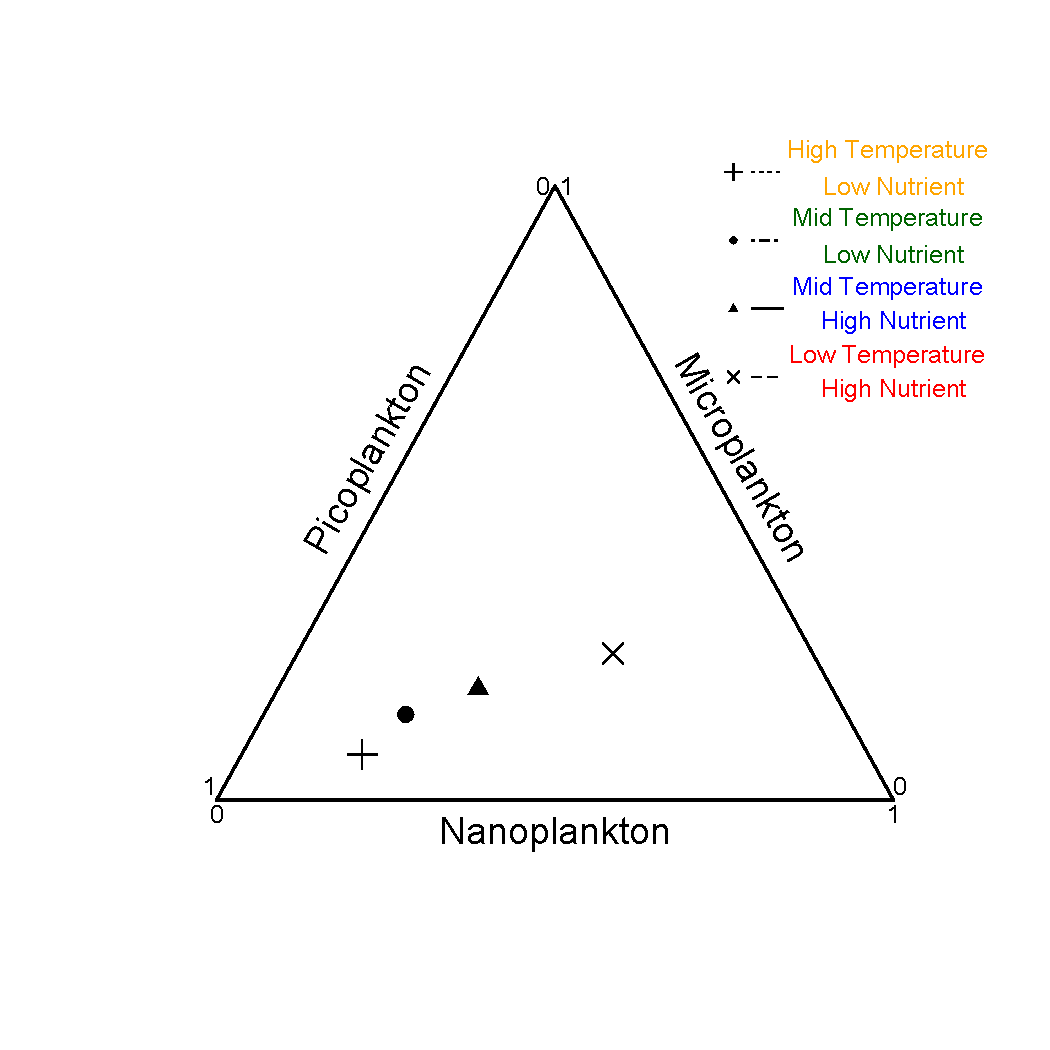
\includegraphics[trim = 10mm 10mm 10mm 10mm, clip,width=0.95\textwidth]{amt_clsEnvFINAL4-6.pdf}}

\end{column}

\begin{column}{0.5\linewidth}

\centering{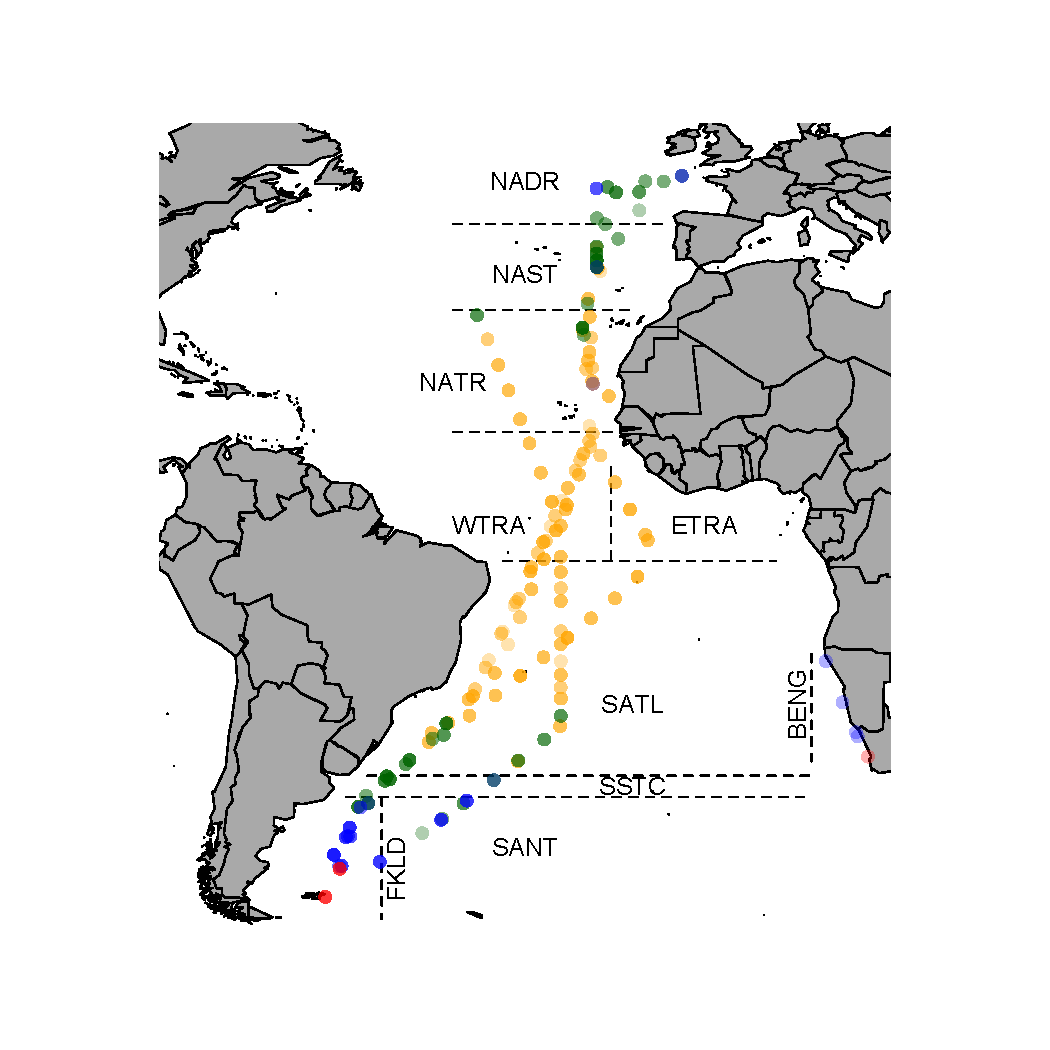
\includegraphics[trim = 20mm 10mm 20mm 20mm, clip,width=0.95\textwidth]{amt_mapClsEnv3-5.pdf}}

\end{column}

\end{columns}

}

\end{frame}
%%% New Slide %%%%
\begin{frame}{Major findings}

\only<1>{

\begin{center}
Environmental selection- Nutrients and Temperature
\end{center}

\begin{columns}[t]

\begin{column}{0.5\linewidth}

\centering{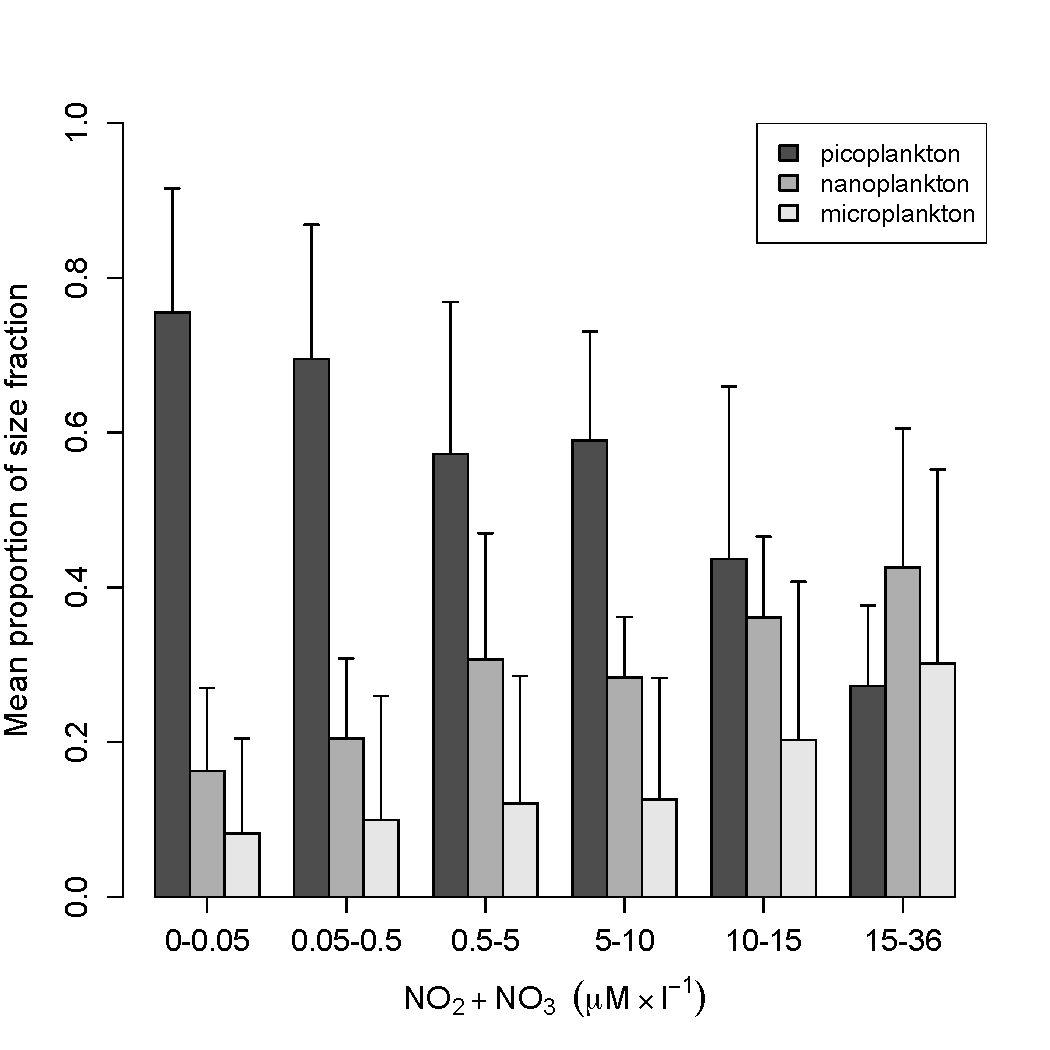
\includegraphics[trim = 0mm 0mm 0mm 15mm, clip,width=.95\textwidth]{amt_NO3_bars2.pdf}}

\end{column}

\begin{column}{0.5\linewidth}

\centering{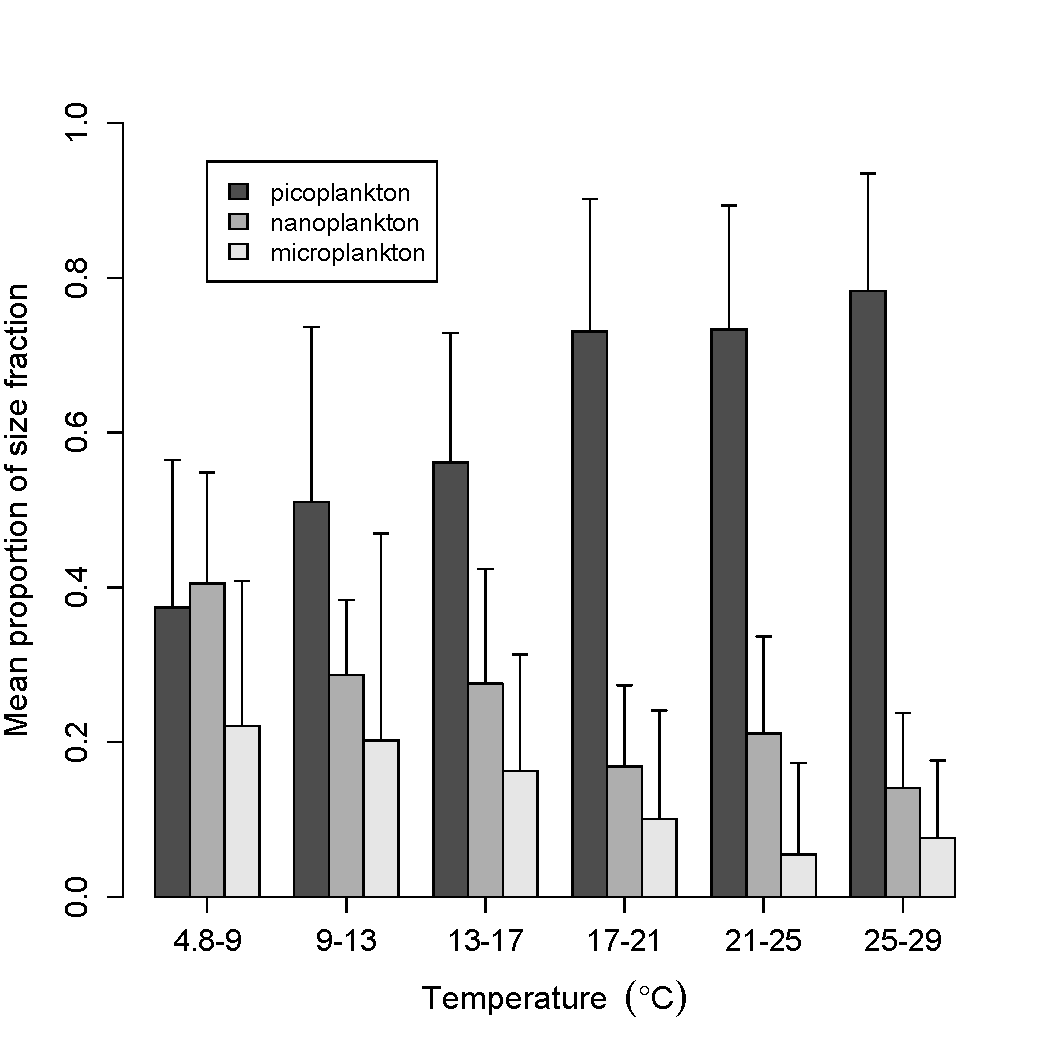
\includegraphics[trim = 0mm 0mm 0mm 15mm, clip,width=.95\textwidth]{amt_Temp_bars2.pdf}}

\end{column}

\end{columns}

}

\only<2>{

\begin{center}
Environmental selection - Grazing pressure
\end{center}

\centering{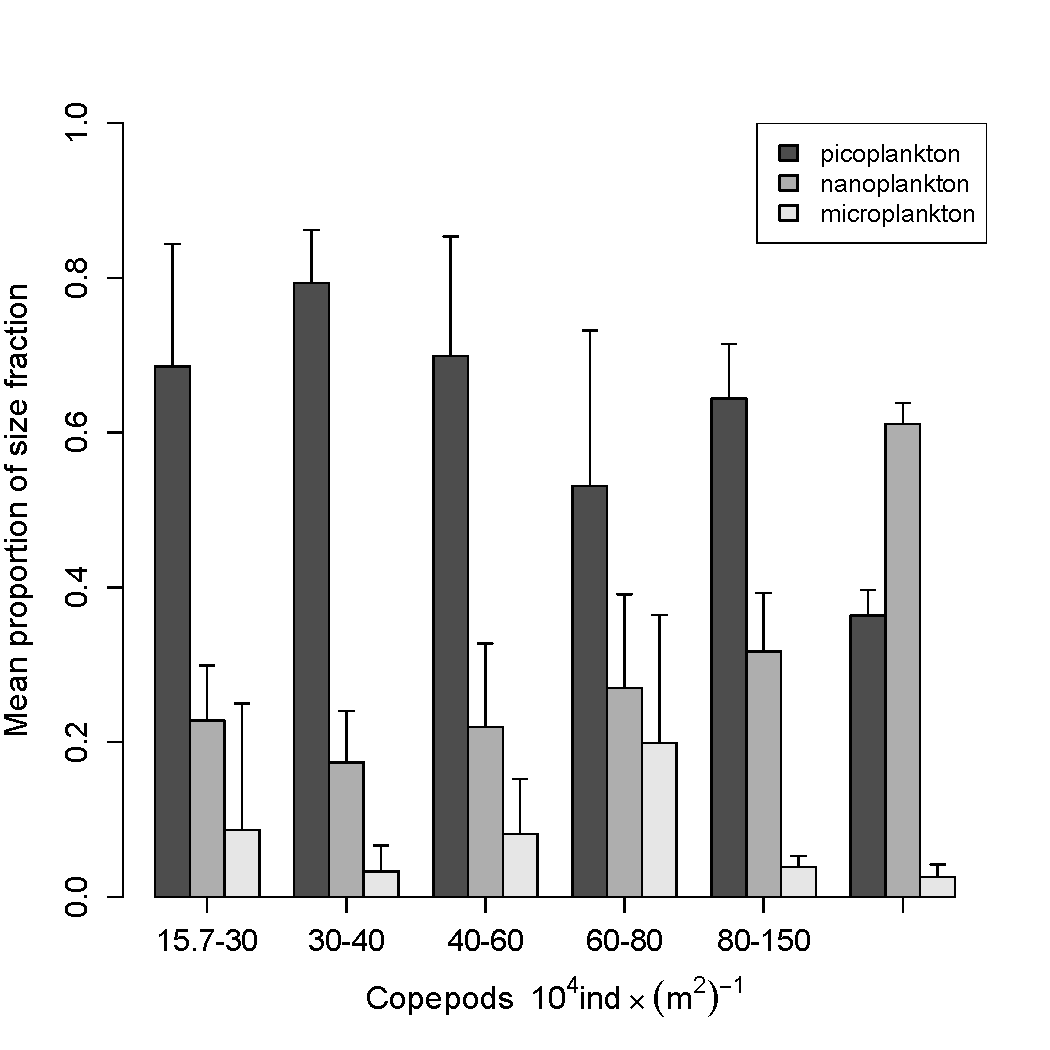
\includegraphics[trim = 0mm 0mm 0mm 15mm, clip,width=0.55\textwidth]{amt_Zoo_bars2.pdf}}

}

\end{frame}
%%% New Slide %%%%
\begin{frame}{Summary}

\begin{itemize}

\item Environmental conditions strongly influence the trait distribution over large scales

\pause

\item Increased trend of mean size fractions in contrasting regions of the Atlantic

\pause

\item Strong bottom-up controls on the phytoplankton community composition

\pause

\item Our analysis captures remarkable features of the cell size variation at an ocean basin scale and irrespective of temporal changes

\end{itemize}

\end{frame}
%%% New Slide %%%%
\section{Phytoplankton size-based model}
\begin{frame}{Phytoplankton size-based model}

\only<1>{

\centering{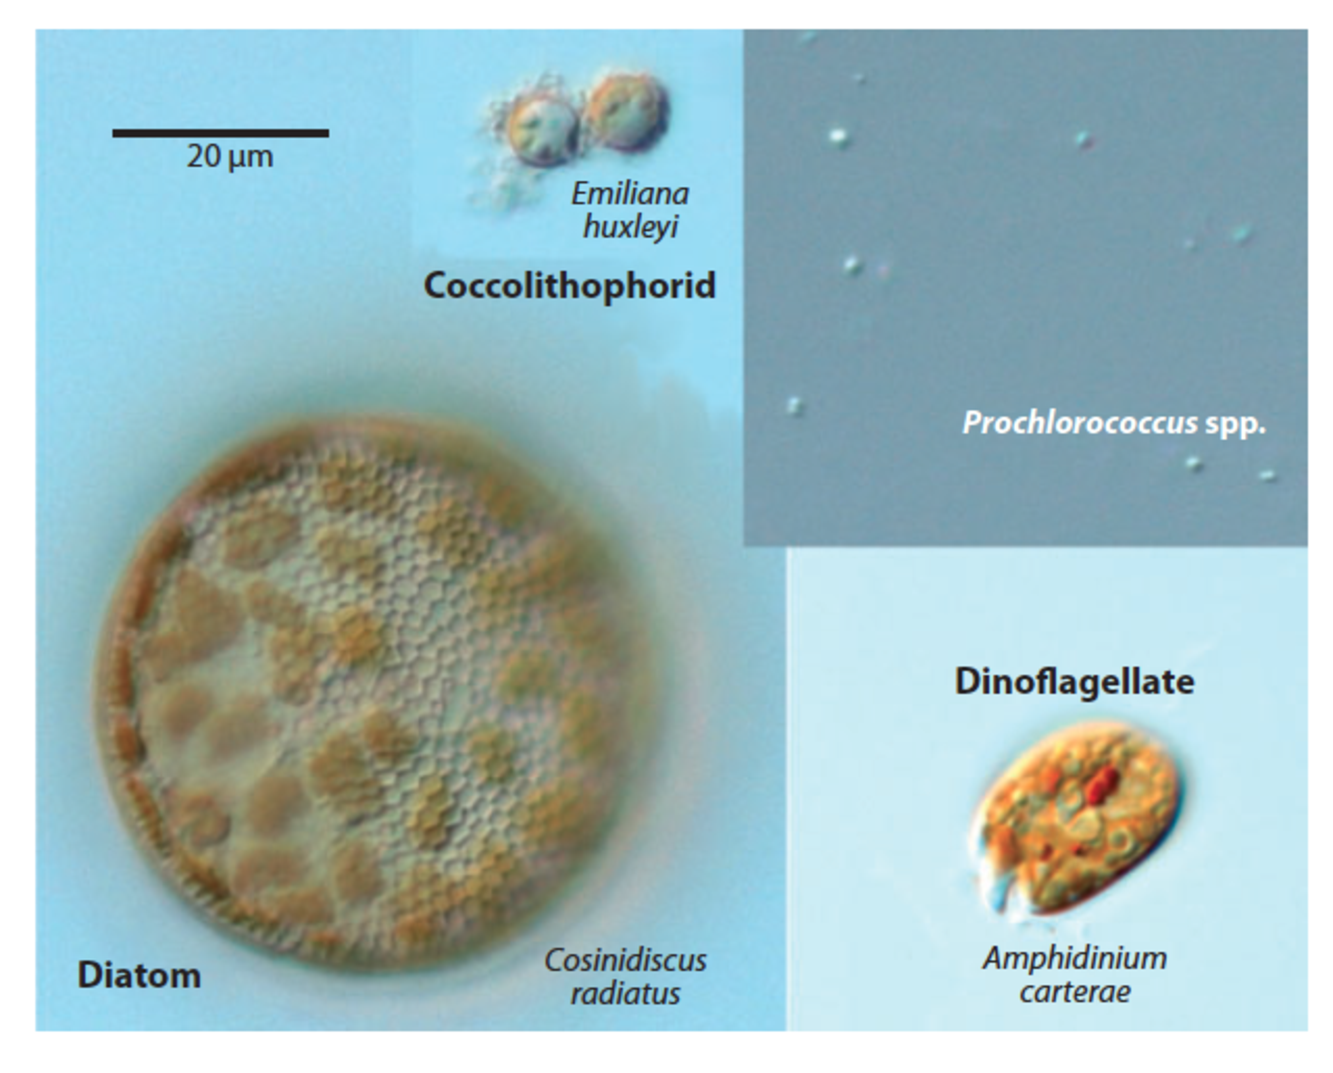
\includegraphics[width=0.7\textwidth]{follows2011-2.pdf}}

\raggedleft {\tiny {Follows and Dutkiewicz, 2011}}

}

\only<2>{

\begin{columns}[t]

\begin{column}{0.5\linewidth}

\vspace{1cm}

\centering{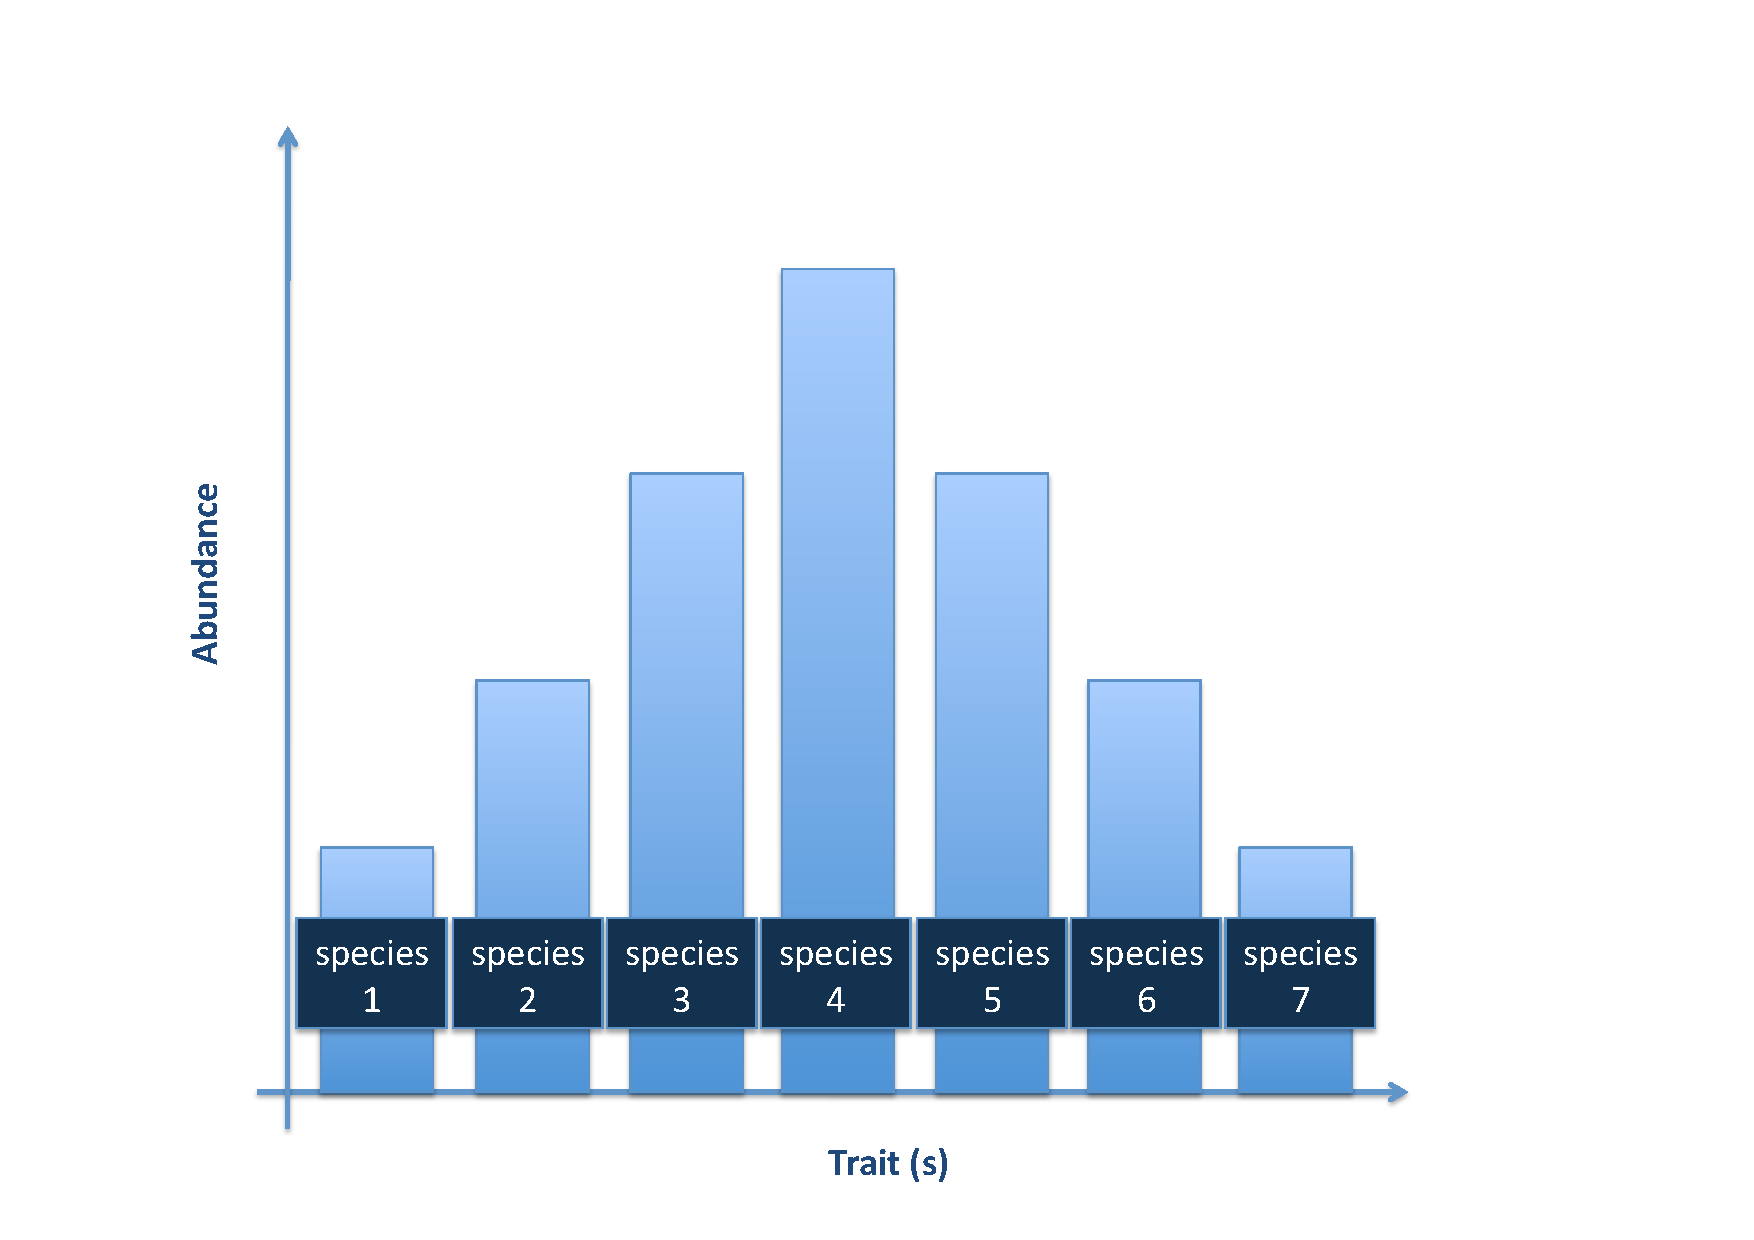
\includegraphics[trim = 5mm 5mm 5mm 20mm, clip,width=1.2\textwidth]{full-ago.pdf}}

\end{column}

\begin{column}{0.5\linewidth}

\begin{block} {Full model}

\begin{eqnarray}
\frac{dP_{1}}{dt} & =  r(s_{1})\,P_{1} \nonumber \\[10pt]
\cdotp \nonumber\\[-10pt]
\cdotp \nonumber\\[-10pt]
\cdotp \nonumber\\[10pt]
\frac{dP_{n}}{dt} & =  r(s_{n})\,P_{n} \nonumber 
\end{eqnarray}

\end{block}

\end{column}

\end{columns}

\raggedleft {\tiny {Merico, 2009}}

}

\only<3>{

\begin{columns}[t]

\begin{column}{0.5\linewidth}

\vspace{1cm}

\centering{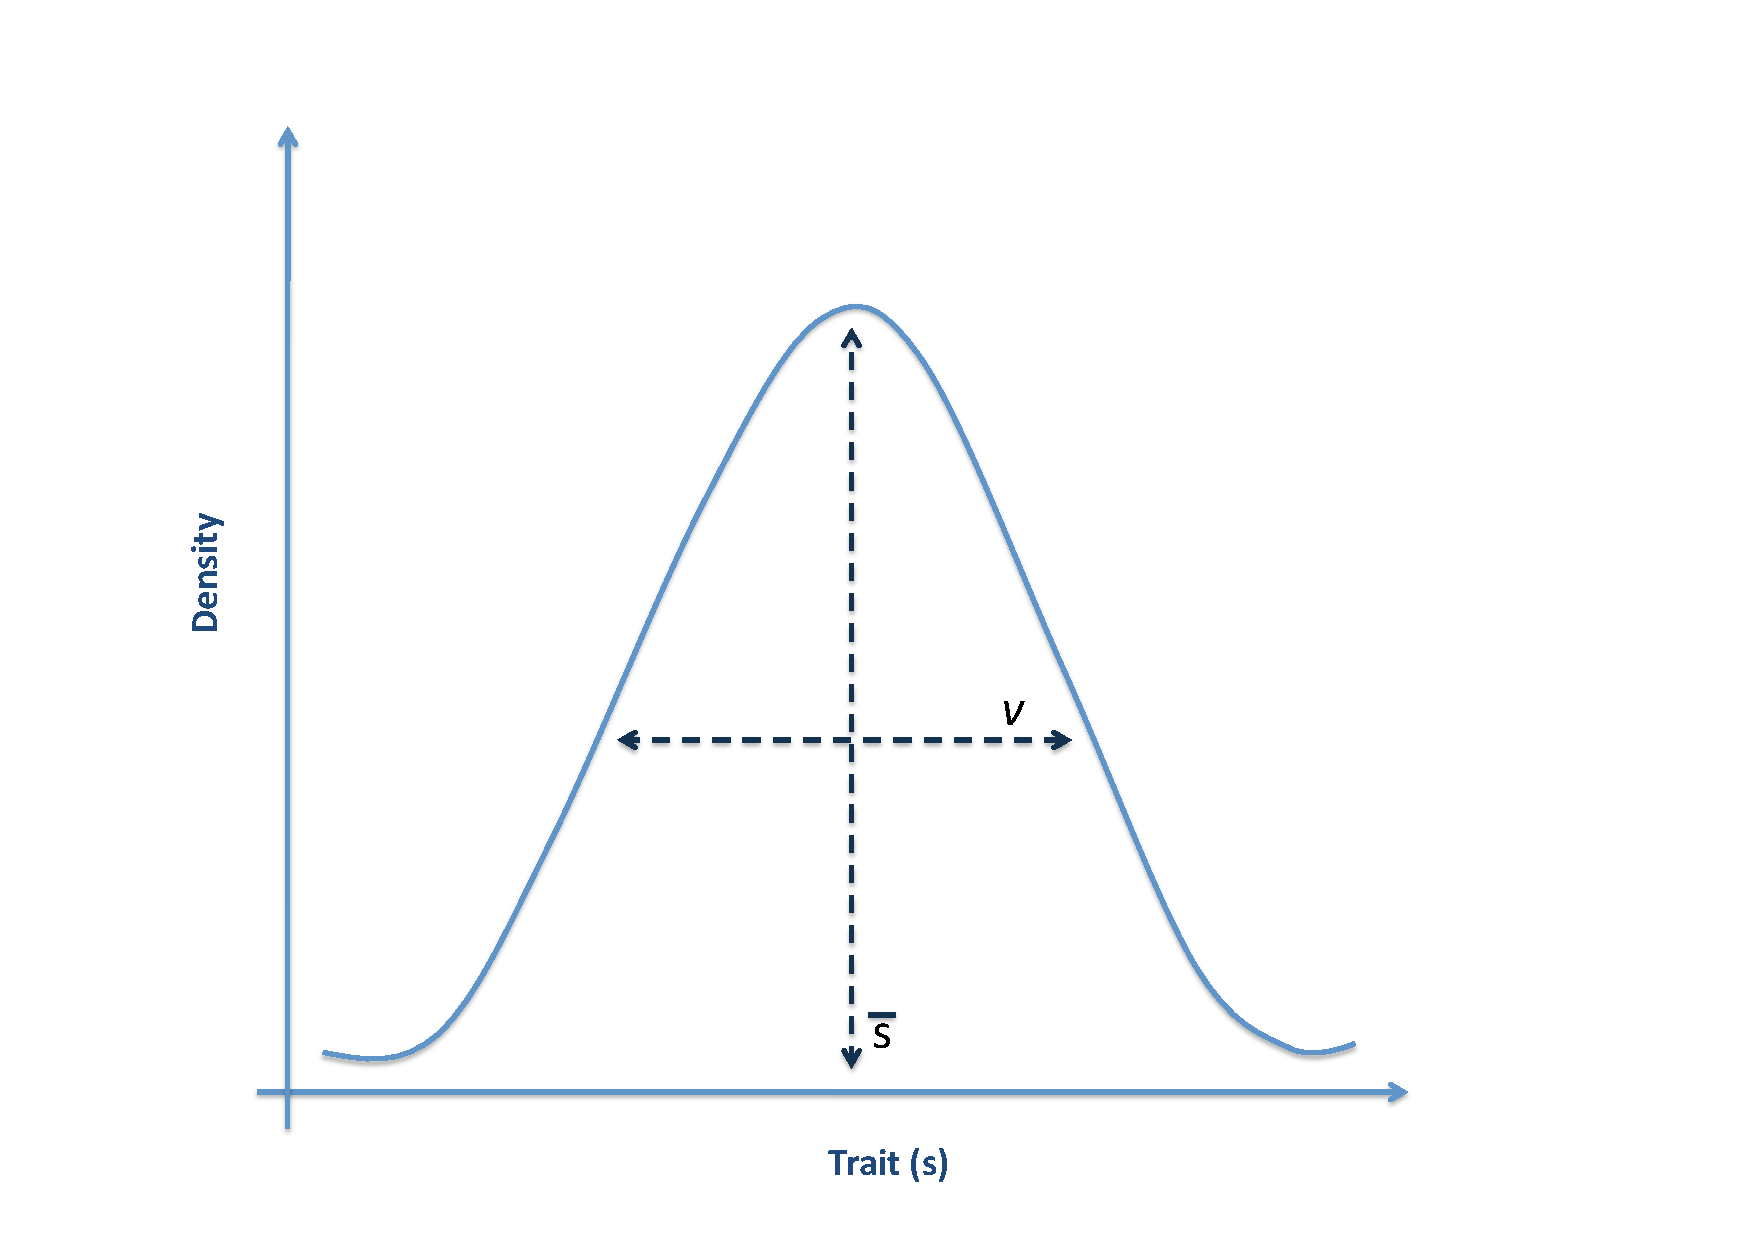
\includegraphics[trim = 5mm 5mm 5mm 20mm, clip,width=1.2\textwidth]{agg-ago.pdf}}

\end{column}

\begin{column}{0.5\linewidth}

\begin{block} {Aggregate model}

\begin{align*}
\frac{dP_{T}}{dt} & = \left[r(\bar{s})+\frac{1}{2}v\frac{\partial^{2} r(\bar{s})}{\partial s^{2}}\right]P_{T} \nonumber \\
& \nonumber \\[-10pt]
\frac{d\bar{s}}{dt} & = v\frac{\partial r(\bar{s})}{\partial s}\nonumber \\
&\nonumber \\[-10pt]
\frac{dv}{dt} & = v^{2}\frac{\partial^{2} r(\bar{s})}{\partial s^{2}}\nonumber\\
\end{align*}

\end{block}

\end{column}

\end{columns}

\raggedleft {\tiny {Merico, 2009}}

}

\only<4>{

\begin{center}
Model Scheme
\end{center}

\centering{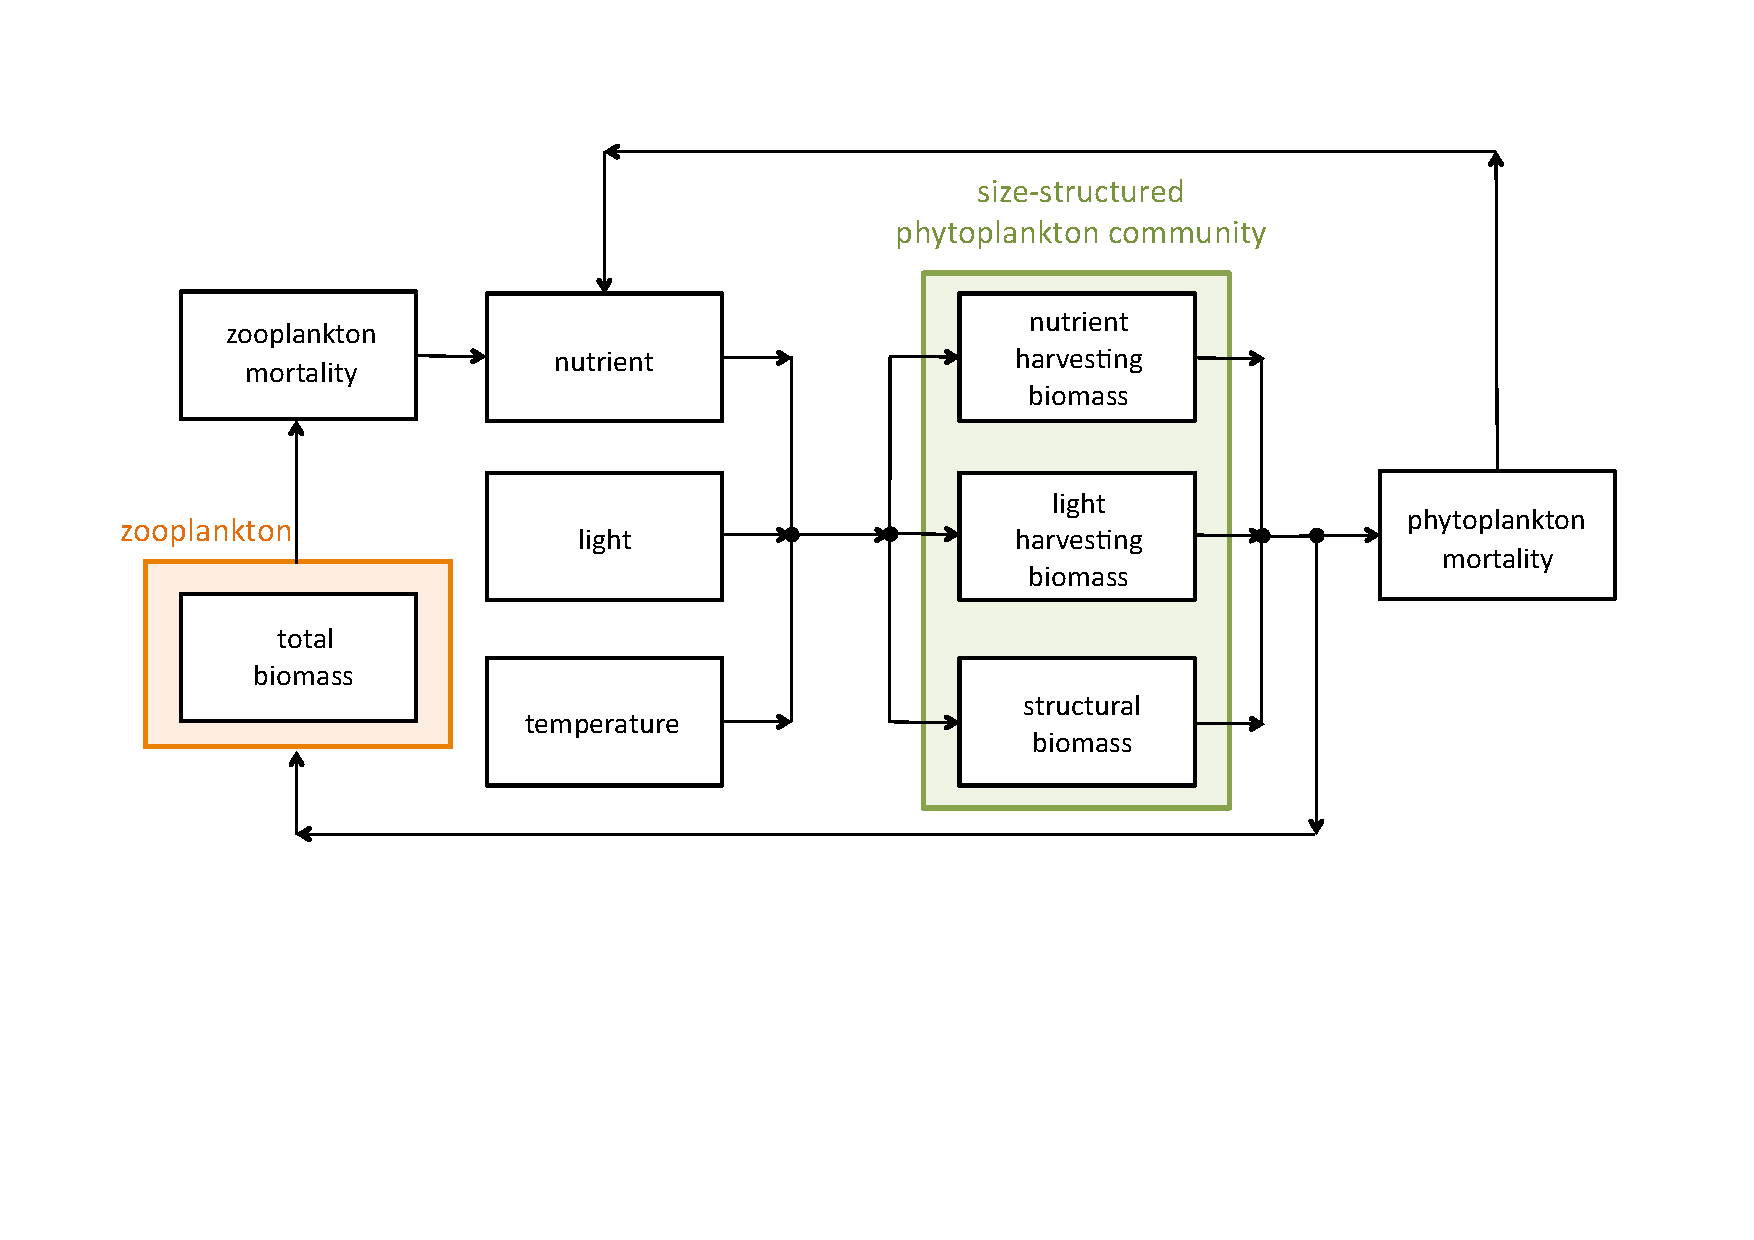
\includegraphics[trim = 0mm 0mm 0mm 0mm, clip,width=1\textwidth]{model-scheme.pdf}}

}

\end{frame}
%%% New Slide %%%%
\section{Phytoplankton and Zooplankton size-based model}
\begin{frame}{Phyto- and Zooplankton size-based model}

\begin{center}
Model Scheme
\end{center}

\centering{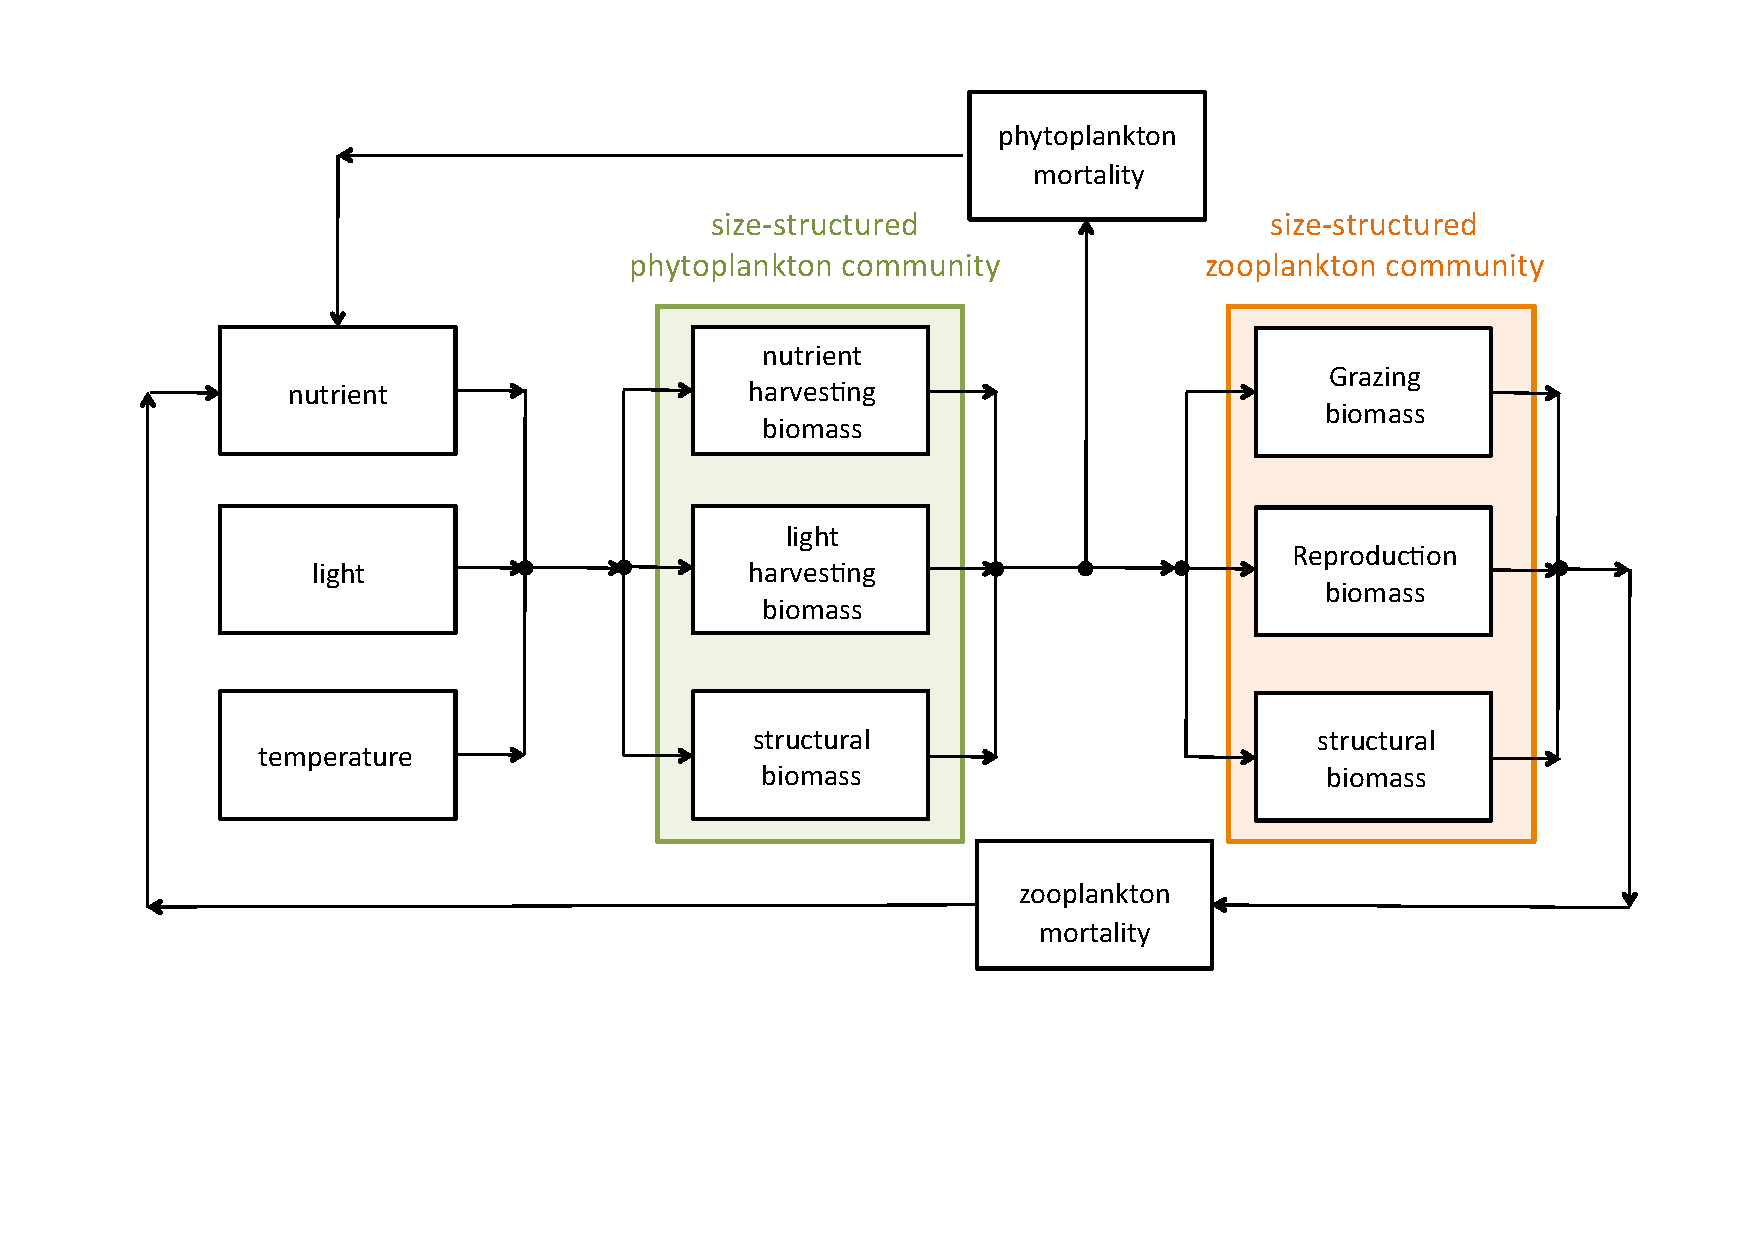
\includegraphics[trim = 0mm 0mm 0mm 0mm, clip,width=1\textwidth]{model-scheme2.pdf}}

\end{frame}
%%% New Slide %%%%
\section{Phytoplankton size evolution}
\begin{frame}{Phytoplankton size evolution}

%\only<1>{

%\centering{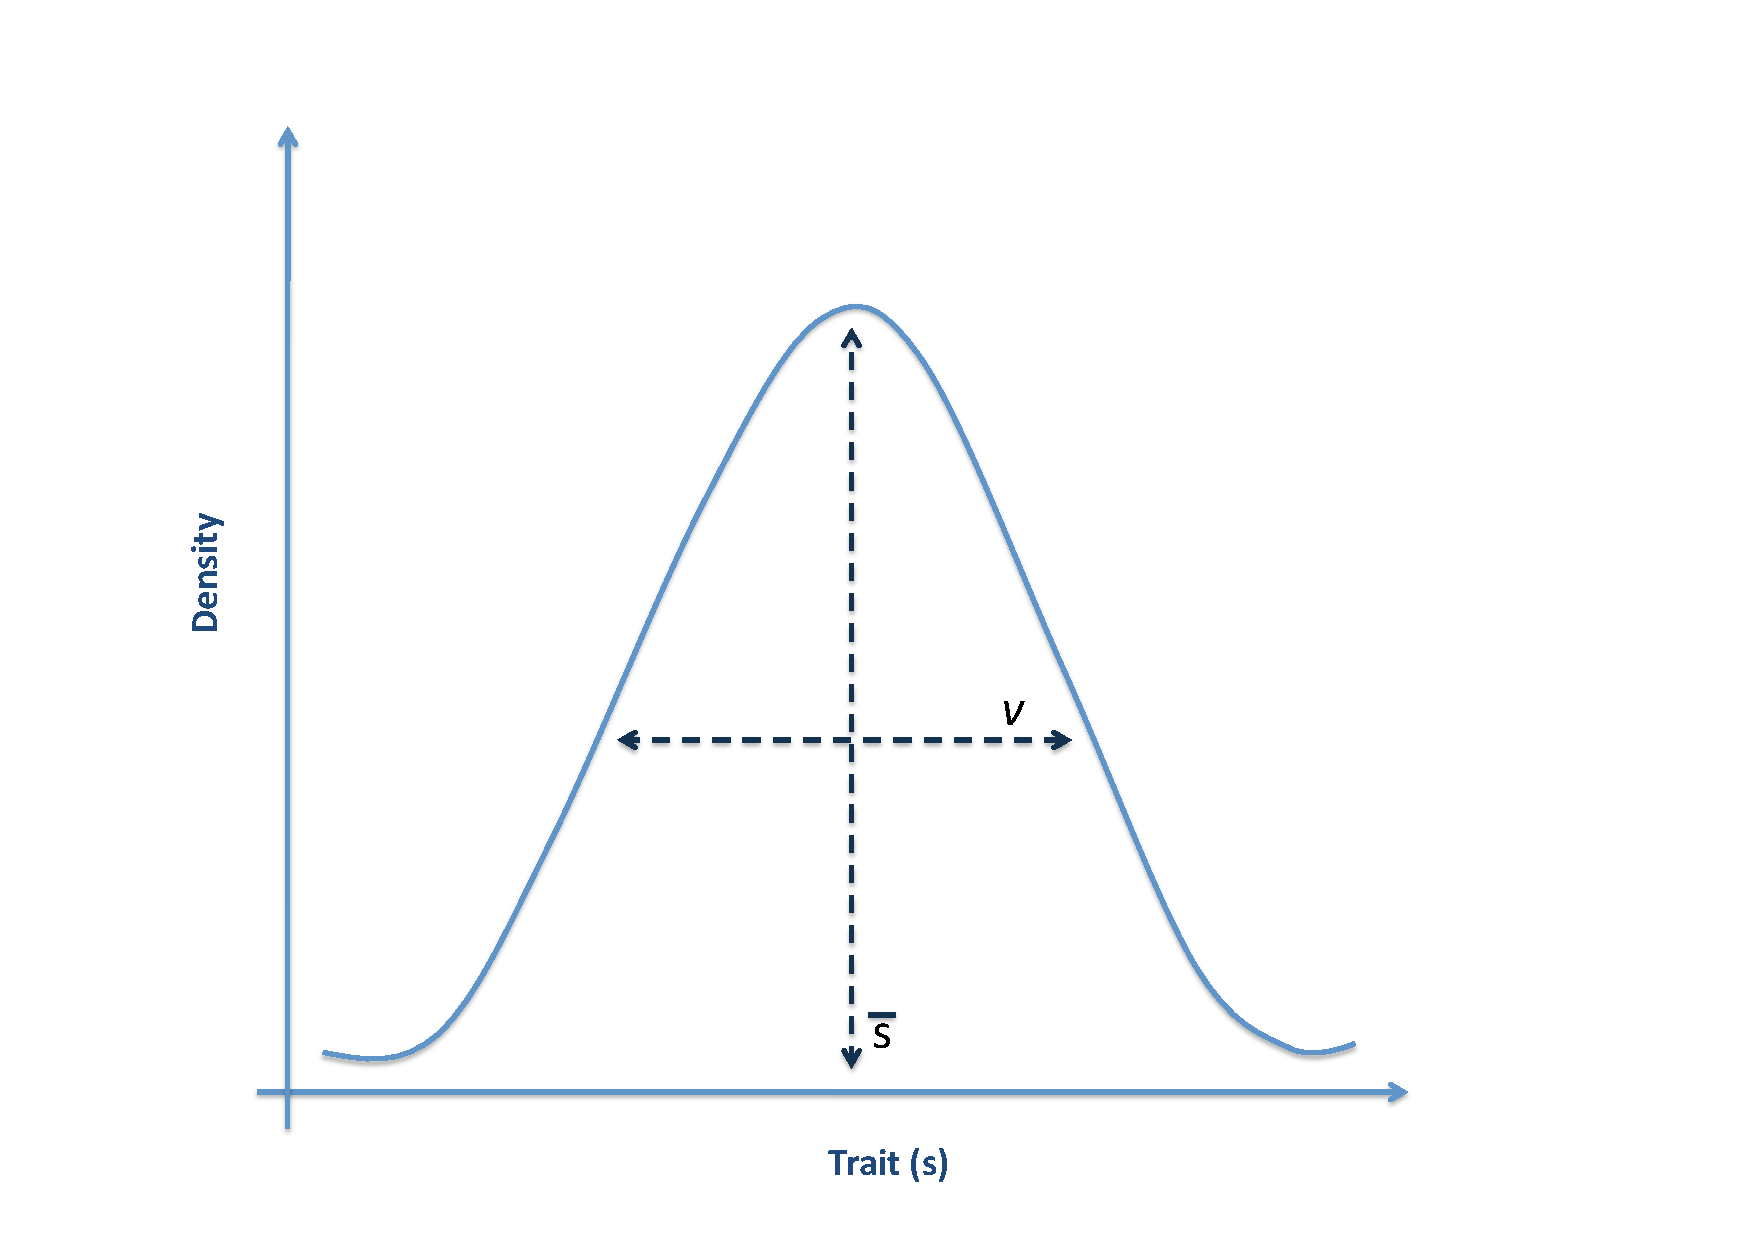
\includegraphics[trim = 5mm 5mm 5mm 20mm, clip,width=1\textwidth]{agg-ago.pdf}}

%}

%\only<2>{

%\centering{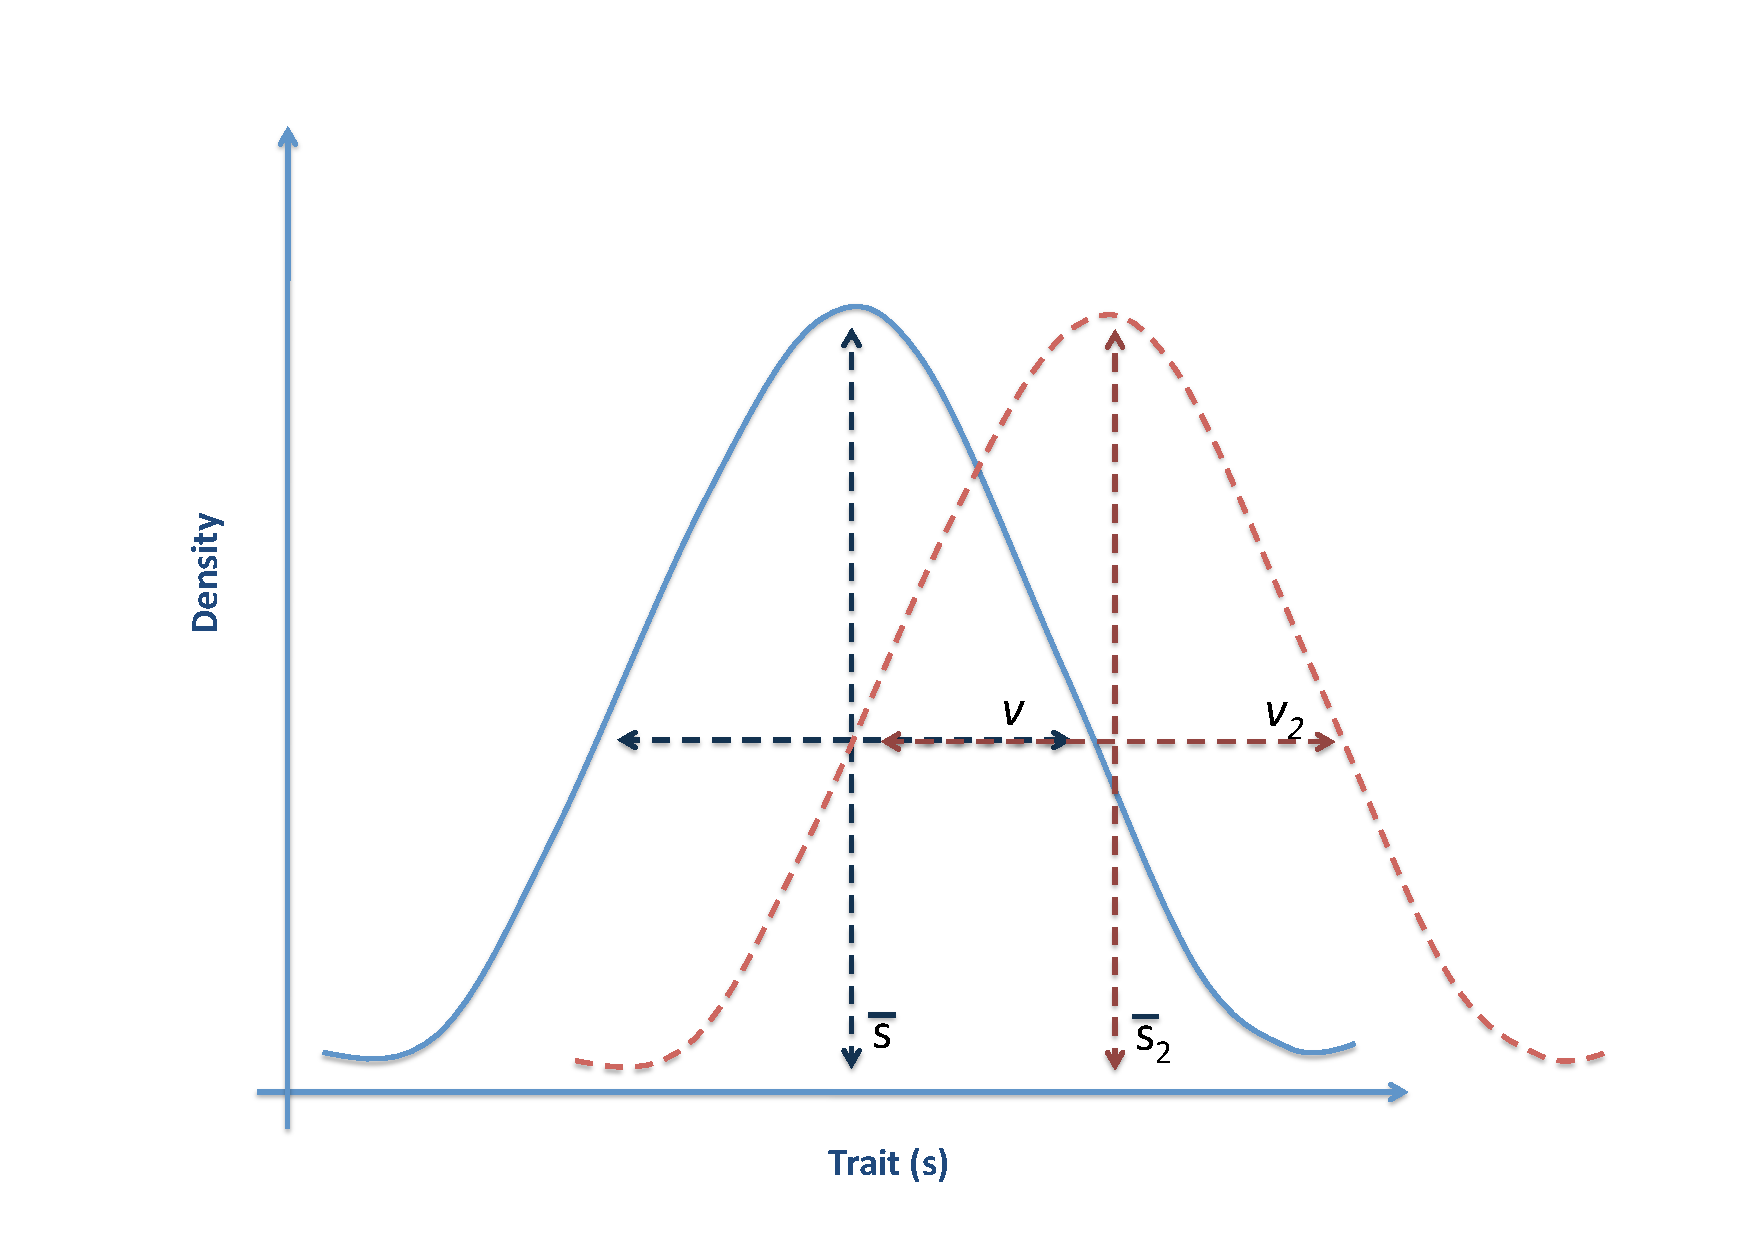
\includegraphics[trim = 5mm 5mm 5mm 20mm, clip,width=1\textwidth]{agg-ago2.pdf}}

%}

%\only<3>{

%\centering{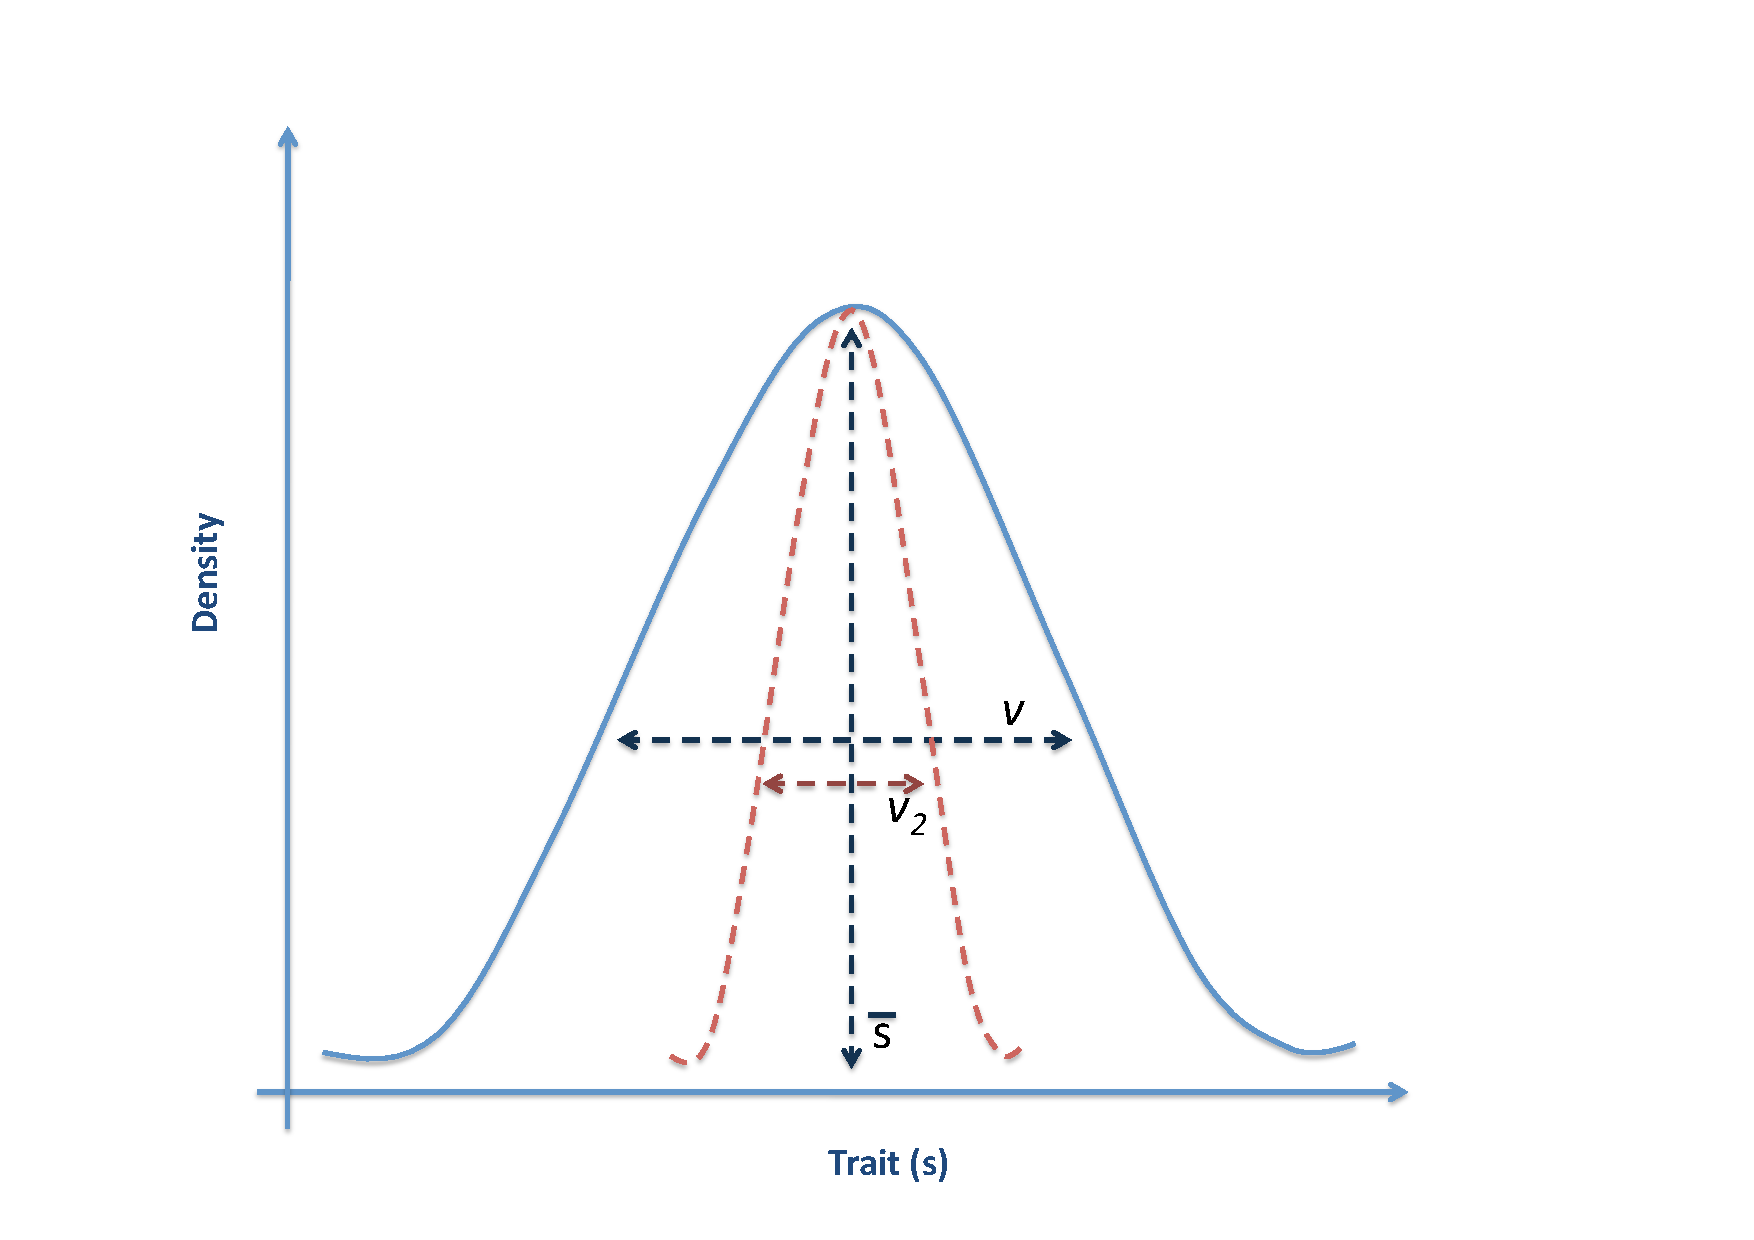
\includegraphics[trim = 5mm 5mm 5mm 20mm, clip,width=1\textwidth]{agg-ago3.pdf}}

%}

\only<1>{ % 4

\centering{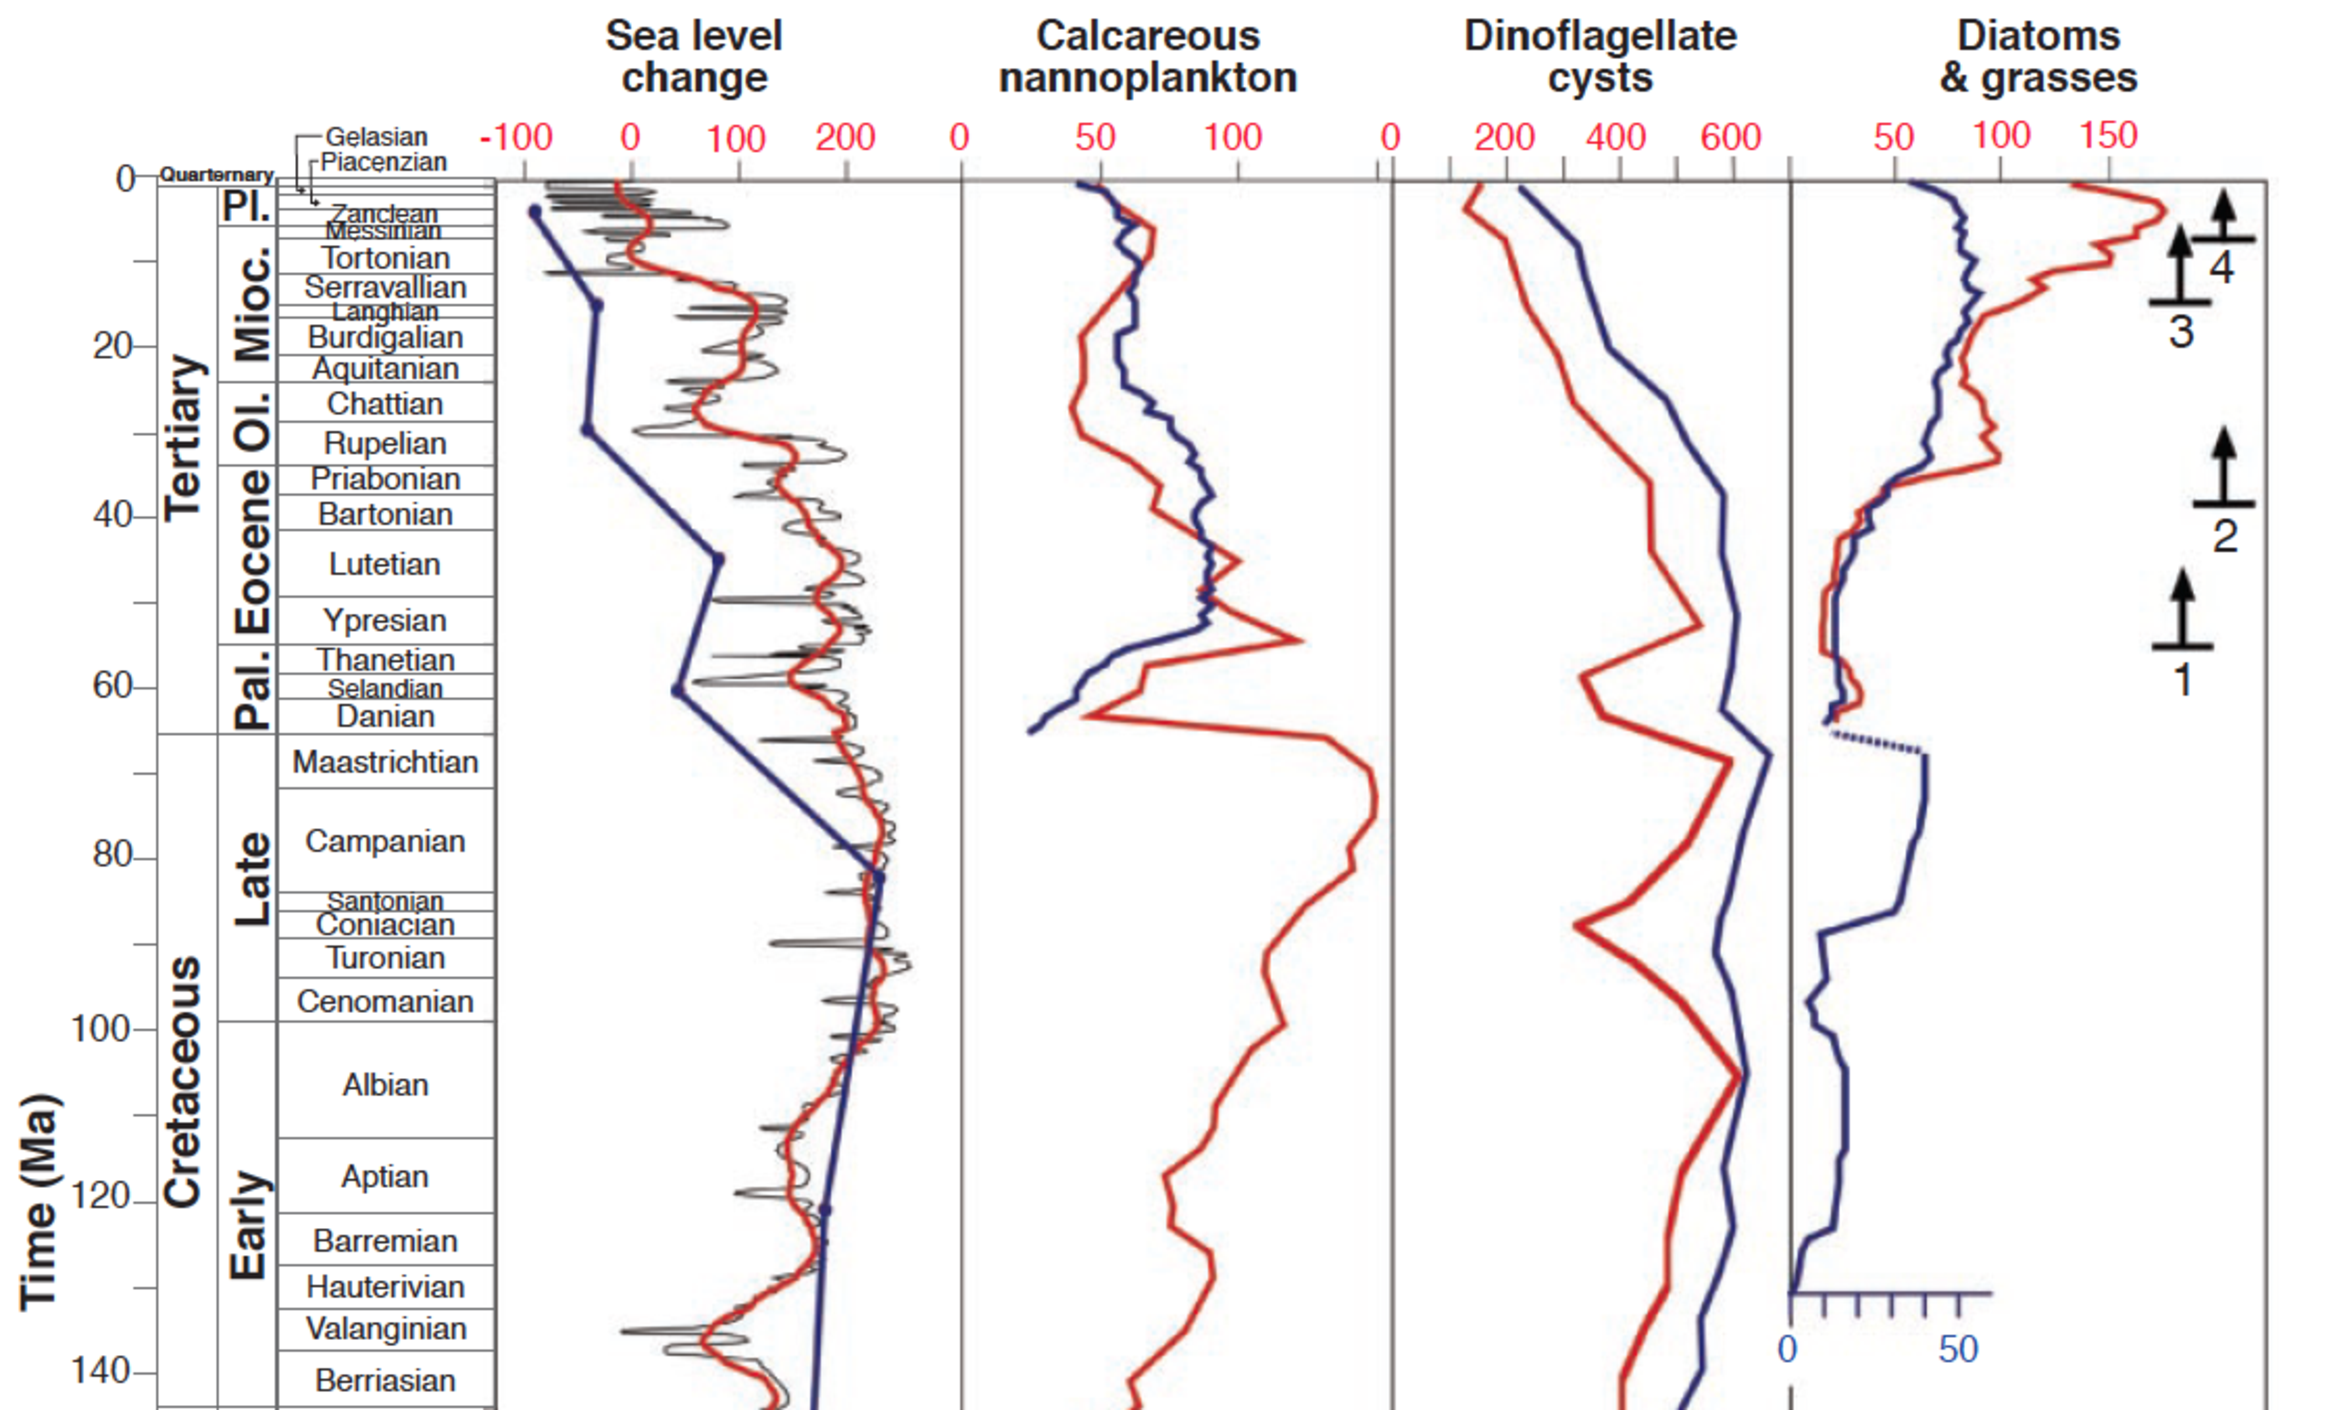
\includegraphics[width=0.9\textwidth]{Falkowski-2004-2.pdf}}

\raggedleft {\tiny {Falkowski, 2004}}

}

\end{frame}
%%% New Slide %%%%
%\begin{frame}{Chronogram}

%\only<1>{

%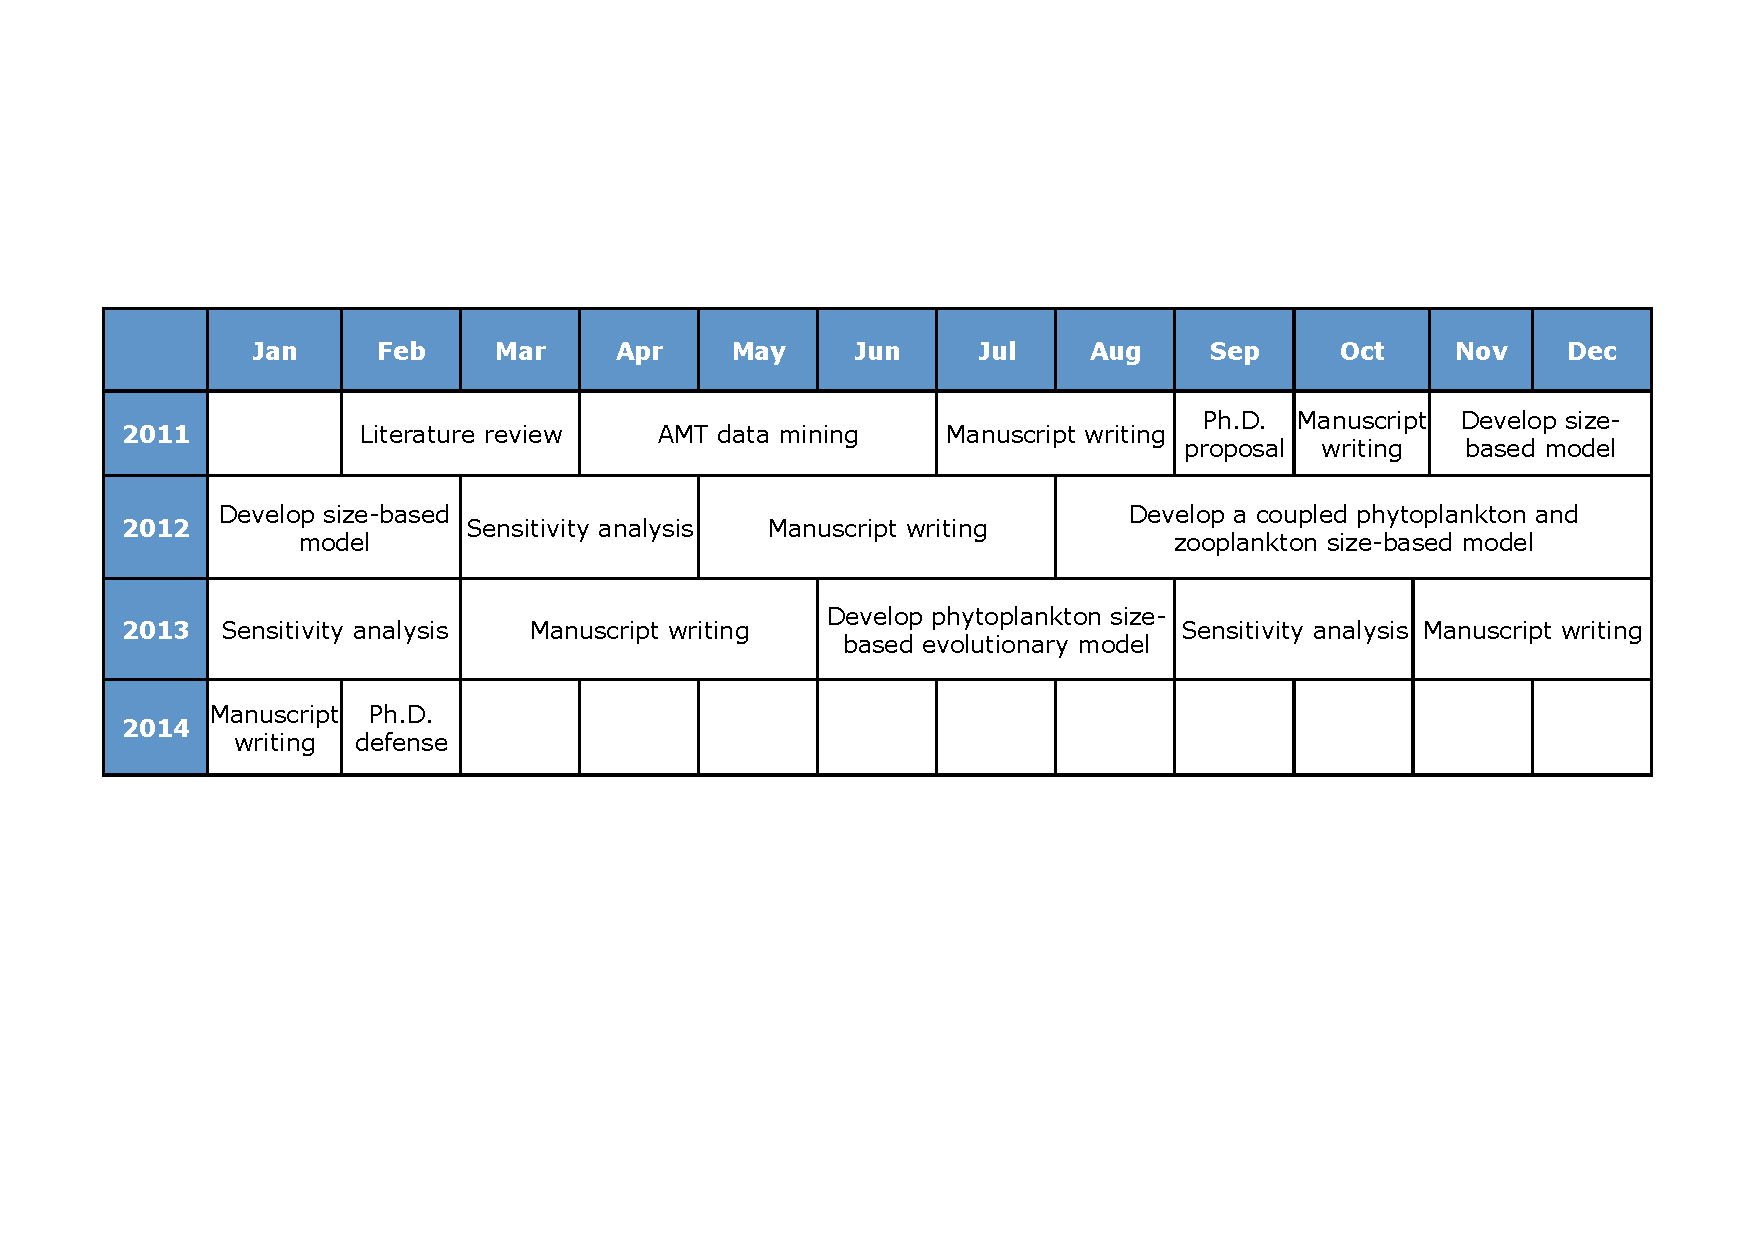
\includegraphics[trim = 15mm 20mm 15mm 20mm, clip, width=\linewidth]{cronogram.pdf}

%}

%\only<2>{

%\centering{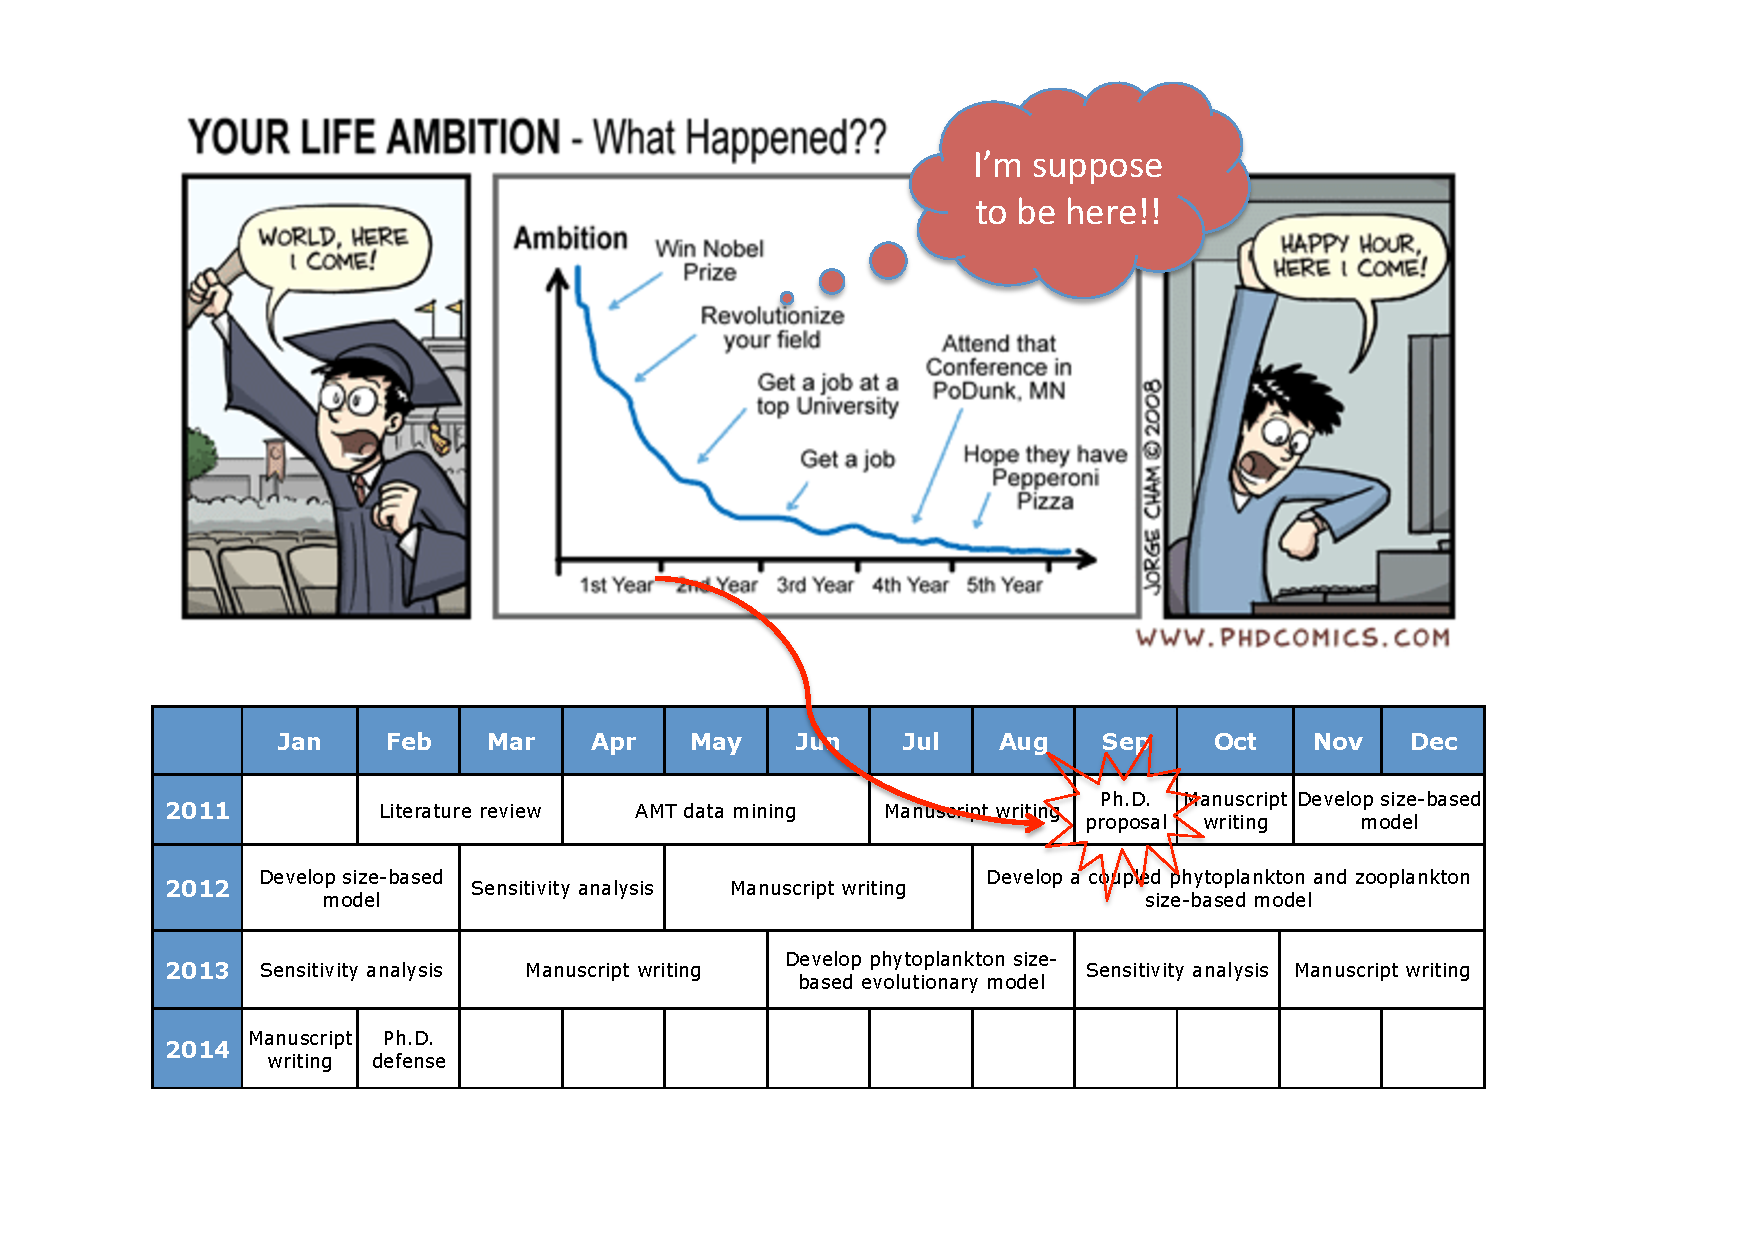
\includegraphics[width=1\textwidth]{chrono_comic.pdf}}

%}

%\end{frame}

\begin{frame}
\centering{\large{Thank you for your attention...}}\\
\vspace{1cm}
\centering{\large{Does size really matters?}}\\
%\centering{
\includegraphics[width=0.5\textwidth]{stormTroopersize.pdf}}\\
\centering{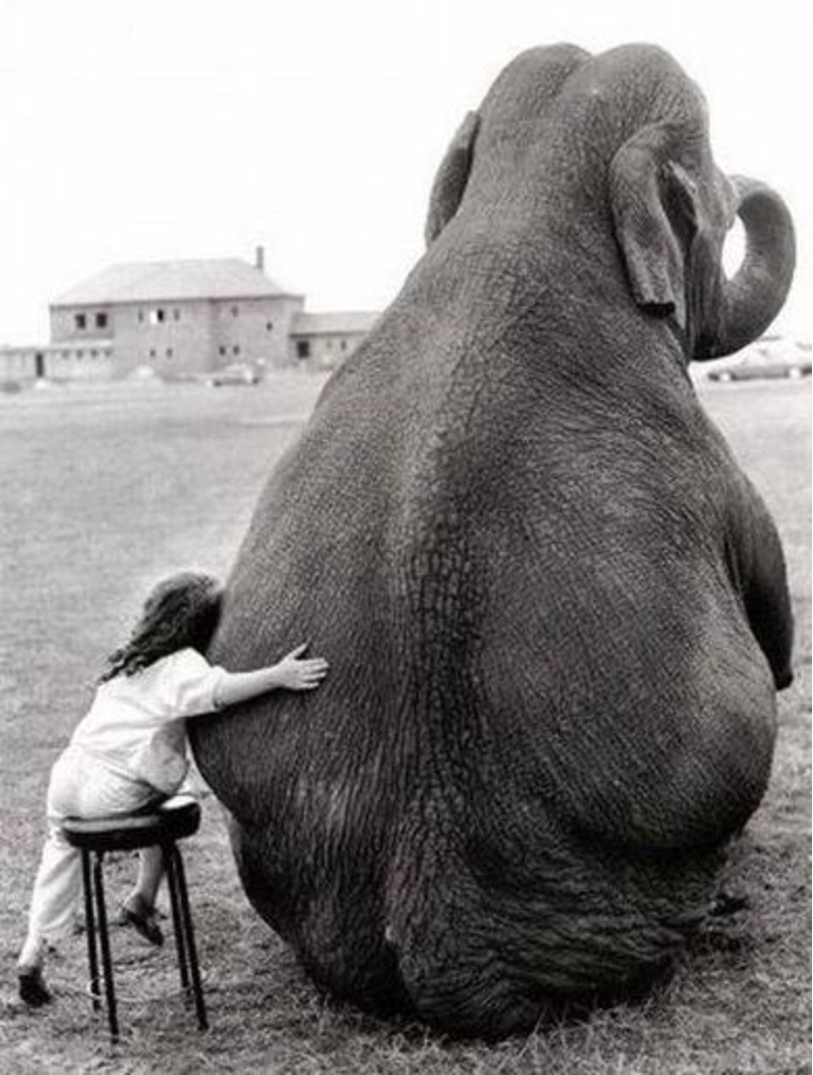
\includegraphics[width=0.3\textwidth]{sizeElephant.pdf}}\\
\centering{\large{In the case of Phytoplankton...Yes it does!!}}\\
\end{frame}

\end{document}